\chapter{Numerical Examples of Sensitivity of Density Estimators}
\label{ch6}

As we have seen from Theorem \ref{theorem-inf-fun-ml-sm-ker-exp-fam} in Chapter \ref{ch5} that, even though the expressions of the influence functions of the penalized ML and SM log-density estimators in $\calQ_{\ker}$ exist, they are hard to be directly used to compare the sensitivities of these density estimators. Instead, we are going to compare their sensitivities numerically, which will be the focus of Section \ref{section-numerical-comparison-sensitivity}. Since we have seen the penalized and early stopping SM density estimators are qualitatively very similar through numerical examples in Chapters \ref{ch3} and \ref{ch4}, we only consider the penalized SM density estimator in this chapter. Since one of the most popular methods of selecting the penalty parameter in the penalized SM density estimation approach is the $K$-fold cross-validation, we turn to studying the sensitivity of the cross-validated penalized SM density estimator in Section \ref{section-sensitivity-cv-penalized-sm-density-estimator}. %We propose a new approach of selecting appropriate values of the penalty parameter depending on the sensitivity in Section \ref{section-sensitivity-choose-penalty-parameter}. 
Since we have both penalized ML and SM density estimators, we discuss in Section \ref{section-which-one-to-use} which density estimator we should use and how to use it. 


\section{Comparison of the Sensitivities of Penalized Maximum Likelihood and Score Matching Density Estimators}\label{section-numerical-comparison-sensitivity}

We study the sensitivities of the penalized ML and SM density estimators numerically in this section. 

The tool we use is the sample influence function defined in Chapter \ref{ch5}. We discuss how to compute the sample influence function of a log-density estimator and that of a density estimator in Section \ref{subsection-computation-sample-inf-fun}. Since we can use either the sample influence function of the log-density estimator or that of the density estimator, we compare them in Section \ref{subsection-sample-inf-fun-logden-vs-den} and show that the former one is a better choice for us. The main comparison of the sensitivities of penalized ML and SM density estimators will be given in Section \ref{subsection-main-comparison-sensitivity}. 

In order to achieve the desired goal, we still define the following maps as we have done in Section \ref{section-influence-function-kernel-exp-fam} in Chapter \ref{ch5}
\begin{align*}
	T_{\lambda} \parens{F} = & \, \log q_{f_{\ML, F}^{\parens{\lambda}}}, && \, \text{ and } && \, S_{\rho} \parens{F} = \log q_{f_{\SM, F}^{\parens{\rho}}}, \\ 
	\widetilde{T}_{\lambda} \parens{F} = & \, q_{f_{\ML, F}^{\parens{\lambda}}}, && \, \text{ and } && \, \widetilde{S}_{\rho} \parens{F} = q_{f_{\SM, F}^{\parens{\rho}}}, 
\end{align*}
where 
\begin{align}
	f_{\ML, F}^{\parens{\lambda}} := & \, \argmin_{f \in \calF} \braces[\bigg]{A (f) - \int_{\mathcal{X}} f (x) \mathrm{d} F (x) + \frac{\lambda}{2} \Vert f \Vert_{\mathcal{H}}^2}, \label{eq-penalized-ml-estimator} \\ 
	f_{\SM, F}^{\parens{\rho}} := & \, \argmin_{f \in \calF} \braces[\bigg]{\frac{1}{2} \langle f, C_{F} f \rangle_{\mathcal{H}} - \langle f, z_{F} \rangle_{\mathcal{H}} + \frac{\rho}{2} \Vert f \Vert_{\mathcal{H}}^2}, \label{eq-penalized-sm-estimator}
\end{align}
with $C_F := \int_{\calX} \sum_{u=1}^d \partial_u k \parens{x, \,\cdot\,} \otimes \partial_u k \parens{x, \,\cdot\,} \diff F \parens{x}$ mapping from $\calH$ to $\calH$, and $z_F := - \int_{\calX} \sum_{u=1}^d \parens{ \partial_u^2 k \parens{x, \,\cdot\,} + \partial_u \log \mu \parens{x} \partial_u k \parens{x, \,\cdot\,}} \diff F \parens{x} \in \calH$. 

In order to ensure the comparability of the penalized ML and SM density estimates, we minimize the objective functionals in \eqref{eq-penalized-ml-estimator} and \eqref{eq-penalized-sm-estimator} over the same finite-dimensional approximating subspace of $\calH$ that is found by the procedures described in Chapter \ref{ch4}, and denote this finalized subspace by $\widetilde{\calH}$. 

\subsection{Computation of the Sample Influence Function}\label{subsection-computation-sample-inf-fun}

We describe how to compute the sample influence function in practice. 

We choose $\varepsilon$ in the definition of the sample influence function to be $\varepsilon_0 := \frac{1}{n+1}$. Then, $\mathrm{SIF}_{x, \varepsilon_0} \parens{T_{\lambda}, F_n, y}$ and $\mathrm{SIF}_{x, \varepsilon_0} \parens{S_{\rho}, F_n, y}$ assess the sensitivity of the penalized ML and SM log-density estimators evaluated at $x$ to the additional observation $y$, respectively; and, similarly, $\mathrm{SIF}_{x, \varepsilon_0} \parens{\widetilde{T}_{\lambda}, F_n, y}$ and $\mathrm{SIF}_{x, \varepsilon_0} \parens{\widetilde{S}_{\rho}, F_n, y}$ assess the sensitivity of the penalized ML and SM density estimators evaluated at $x$ to the additional observation $y$, respectively. 

Algorithm \ref{algo-sample-inf-fun-ml} describes how to compute $\mathrm{SIF}_{x, \varepsilon_0} \parens{T_{\lambda}, F_n, y}$; if one would like to compute $\mathrm{SIF}_{x, \varepsilon_0} \parens{\widetilde{T}_{\lambda}, F_n, y}$, simply do not take the logarithm in Steps \ref{algo-sample-inf-fun-ml-2} and \ref{algo-sample-inf-fun-ml-3}. 

\begin{algorithm}
\caption{Computation of $\mathrm{SIF}_{x, \varepsilon_0} \parens{T_{\lambda}, F_n, y}$}\label{algo-sample-inf-fun-ml}
\begin{algorithmic}[1]
\Statex \algorithmicrequire 
\begin{itemize}\setlength\itemsep{0em}
	\item $X_1, \cdots, X_n$, data; 
	\item $y \in \calX$, contaminant; 
	\item $\lambda > 0$, penalty parameter; 
	\item $\widetilde{\calH}$, the finite-dimensional approximating subspace over which we minimize the penalized NLL loss functional; 
	\item $\sets{x_{\ell}}_{\ell=1}^L \subset \calX$, a set of evaluation points. 
\end{itemize}

\vspace{5pt}

\State Compute $f_{\ML, F_n}^{\parens{\lambda}}$ and $f_{\ML, \parens{1 - \varepsilon_0} F_n + \varepsilon_0 \delta_y}^{\parens{\lambda}}$%, the minimizers of the penalized NLL loss functional over $\widetilde{\calH}$ under different empirical distributions, 
	using Algorithm \ref{algo-nll-full-gd-algo} in Chapter \ref{ch4}; 
\State Compute $\log q_{f_{\ML, F_n}^{\parens{\lambda}}} \parens{x_{\ell}}$ and $\log q_{f_{\ML, \parens{1 - \varepsilon_0} F_n + \varepsilon_0 \delta_y}^{\parens{\lambda}}} \parens{x_{\ell}}$ for all $\ell = 1, \cdots, L$; \label{algo-sample-inf-fun-ml-2}
\State Compute \label{algo-sample-inf-fun-ml-3}
\begin{align*}
	\parens[\Big]{\log q_{f_{\ML, \parens{1 - \varepsilon_0} F_n + \varepsilon_0 \delta_y}^{\parens{\lambda}}} \parens{x_{\ell}} - \log q_{f_{\ML, F_n}^{\parens{\lambda}}} \parens{x_{\ell}}} \times \parens{n+1}, \qquad \text{ for all } \ell = 1, \cdots, L; 
\end{align*}
\State \textbf{return} the results from Step \ref{algo-sample-inf-fun-ml-3}. 
\end{algorithmic}
\end{algorithm}

Similarly, Algorithm \ref{algo-sample-inf-fun-sm} describes how to compute $\mathrm{SIF}_{x, \varepsilon_0} \parens{S_{\rho}, F_n, y}$; if one would like to compute $\mathrm{SIF}_{x, \varepsilon_0} \parens{\widetilde{S}_{\rho}, F_n, y}$, do not take the logarithm in Steps \ref{algo-sample-inf-fun-sm-2} and \ref{algo-sample-inf-fun-sm-3}. 

\begin{algorithm}
\caption{Computation of $\mathrm{SIF}_{x, \varepsilon_0} \parens{S_{\rho}, F_n, y}$}\label{algo-sample-inf-fun-sm}
\begin{algorithmic}[1]
\Statex \algorithmicrequire 
\begin{itemize}\setlength\itemsep{0em}
	\item $X_1, \cdots, X_n$, data; 
	\item $y \in \calX$, contaminant; 
	\item $\rho > 0$, penalty parameter; 
	\item $\widetilde{\calH}$, the finite-dimensional approximating subspace over which we minimize the penalized SM loss functional; 
	\item $\sets{x_{\ell}}_{\ell=1}^L \subset \calX$, a set of evaluation points. 
\end{itemize}

\vspace{5pt}

\State Compute $f_{\SM, F_n}^{\parens{\rho}}$ and $f_{\SM, \parens{1 - \varepsilon_0} F_n + \varepsilon_0 \delta_y}^{\parens{\rho}}$
%, the minimizers of the penalized SM loss functional over $\widetilde{\calH}$ under different empirical distributions, 
using Proposition \ref{prop-penalized-sm-fin-dim-space} in Chapter \ref{ch4}; 
\State Compute $\log q_{f_{\SM, F_n}^{\parens{\rho}}} \parens{x_{\ell}}$ and $\log q_{f_{\SM, \parens{1 - \varepsilon_0} F_n + \varepsilon_0 \delta_y}^{\parens{\rho}}} \parens{x_{\ell}}$ for all $\ell = 1, \cdots, L$; \label{algo-sample-inf-fun-sm-2} 
\State Compute \label{algo-sample-inf-fun-sm-3}
\begin{align*}
	\parens[\Big]{\log q_{f_{\SM, \parens{1 - \varepsilon_0} F_n + \varepsilon_0 \delta_y}^{\parens{\rho}}} \parens{x_{\ell}} - \log q_{f_{\SM, F_n}^{\parens{\rho}}} \parens{x_{\ell}}} \times \parens{n+1}, \qquad \text{ for all } \ell = 1, \cdots, L; 
\end{align*}
\State \textbf{return} the results from Step \ref{algo-sample-inf-fun-sm-3}. 
\end{algorithmic}
\end{algorithm}

\subsection{Comparison of the Sample Influence Functions of Log-density and Density Estimators}\label{subsection-sample-inf-fun-logden-vs-den}

Our goal of the current section is to show, between the sample influence function of the log-density estimator and that of the density estimator in $\calQ_{\ker}$, the former is the better choice for us. 

We first use numerical examples to demonstrate this. We still use the \texttt{waiting} variable in the Old Faithful Geyser dataset but remove the original isolated observation 108 therein. This is to avoid the interaction between 108 and the additional observation $y$. We use the same $\calX$, $k$, $\mu$, and $\widetilde{\calH}$ as those in Chapter \ref{ch4}. 

We focus on the penalized SM density estimator for now. Fix $\rho = e^{-11}$. Figure \ref{fig-inffun-logdensity-vs-density-sm-y=120} shows the penalized SM log-density and density estimates with and without $y = 120$ and the corresponding sample influence functions, and Figure \ref{fig-inffun-logdensity-vs-density-sm-y=180} shows the penalized SM log-density and density estimates with and without $y = 180$ and the corresponding sample influence functions. Recall that we choose $\mu$ to be the pdf of the Gamma distribution with the shape and scale parameters to be 36 and 2, respectively, and $\mu \parens{x} \to 0$ and $\log \mu \parens{x} \to -\infty$ as $x \to \infty$. Then, comparing Panel [D] in Figure \ref{fig-inffun-logdensity-vs-density-sm-y=120} and that in Figure \ref{fig-inffun-logdensity-vs-density-sm-y=180}, we see that, when $y$ is large, the spike in the penalized SM density estimate may disappear due to this particular choice of $\mu$. The sample influence function of the penalized SM density estimator may fail to capture the bump or the spike in the penalized SM density estimate when an isolated observation is present (see Panel [F] in Figure \ref{fig-inffun-logdensity-vs-density-sm-y=180}). In other words, understanding the sensitivity of the penalized SM density estimator via the sample influence function of the density estimator can be misleading. %Numerical examples of the penalized ML density estimator also confirm this; see Figures \ref{fig-inffun-logdensity-vs-density-ml-y=120} and Figure \ref{fig-inffun-logdensity-vs-density-ml-y=180} for evidence. 

However, the issue with the sample influence function of the density estimator described above does \emph{not} occur to the sample influence function of the log-density estimator. Comparing Panel [C] in Figure \ref{fig-inffun-logdensity-vs-density-sm-y=120} and that in Figure \ref{fig-inffun-logdensity-vs-density-sm-y=180}, we see the sample influence function of the penalized SM log-density estimator succeeds in capturing the spike at the isolated observation, no matter how far $y$ is from the bulk of the data. Numerical examples of the penalized ML density estimator also confirm this; see Figures \ref{fig-inffun-logdensity-vs-density-ml-y=120} and Figure \ref{fig-inffun-logdensity-vs-density-ml-y=180} for evidence. 

\begin{figure}% [h!]
	\centering 
	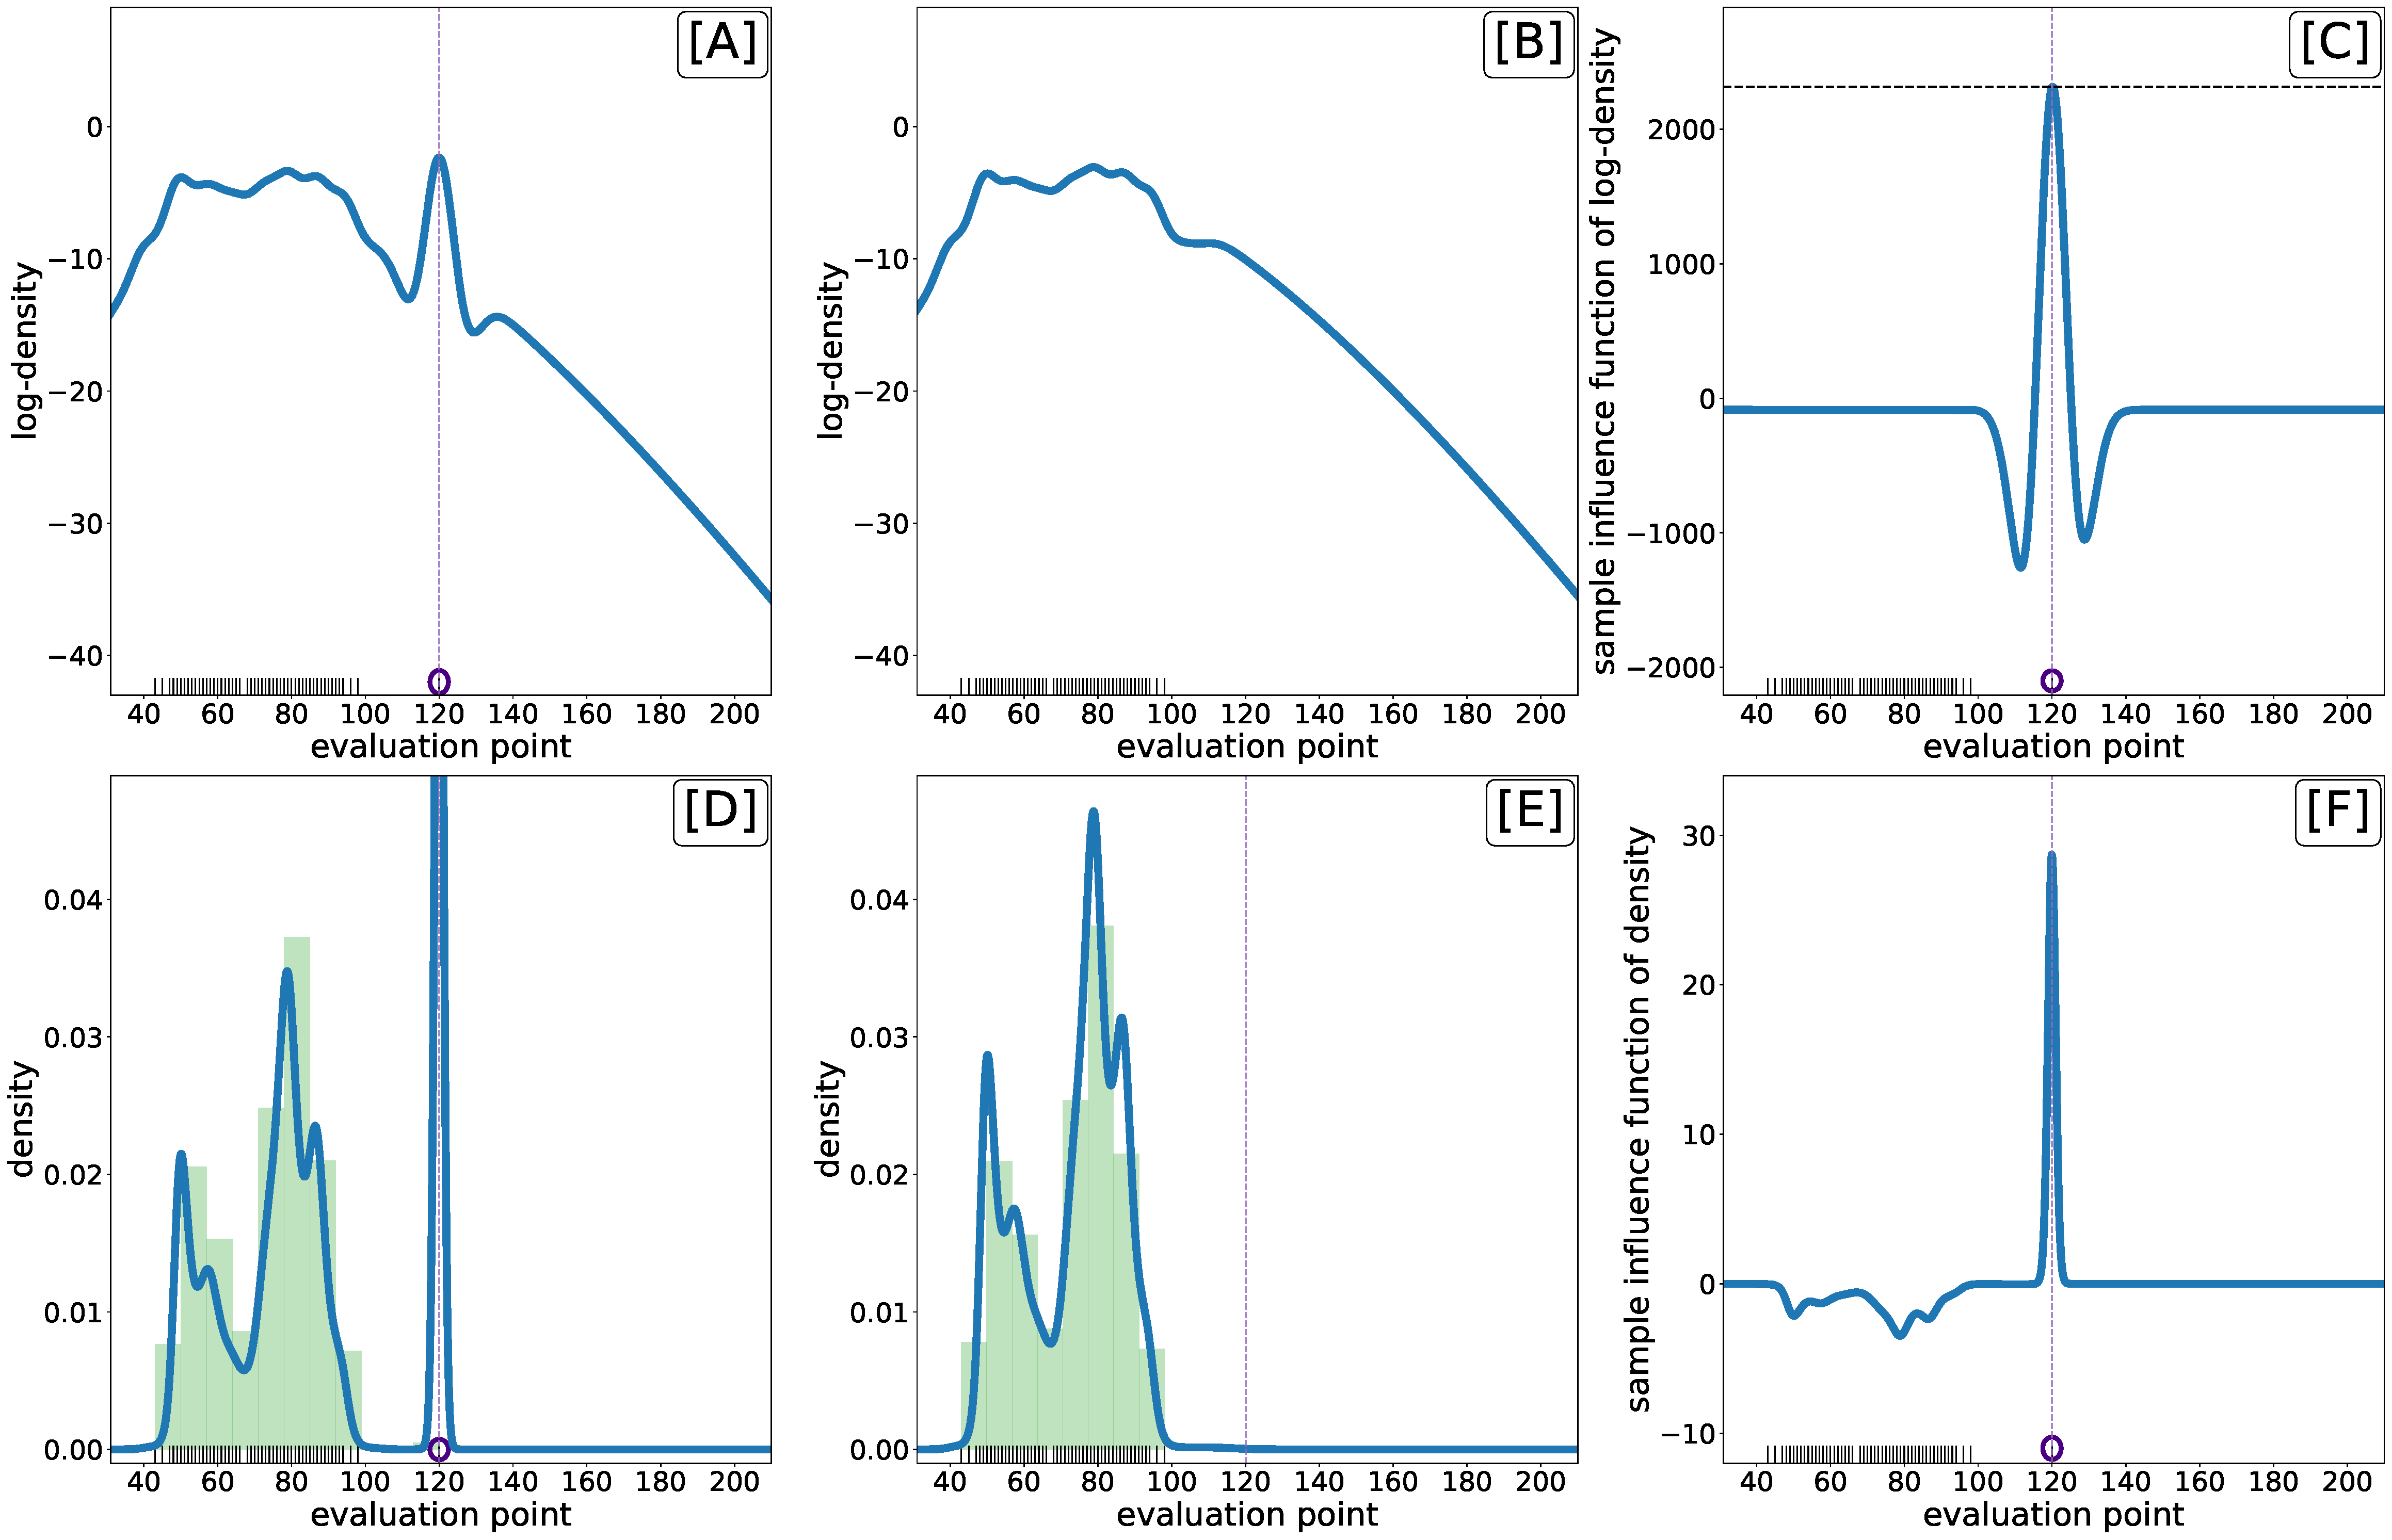
\includegraphics[width=\textwidth]{../plots/comparison-inffunden-inffunlogden-logdensity-density-contam-sm-logpenparam=-11.0-data=120.0-gamma-36.0-2.0.pdf}
	\caption{Fix $\rho = e^{-11}$. Panels [A] and [B] show the penalized SM log-density estimates with and without the additional observation $y = 120$, respectively. Panel [C] shows the sample influence function of the log-density estimator. Panels [D] and [E] show the penalized SM density estimates with and without the additional observation $y = 120$, respectively. Panel [F] shows the sample influence function of the density estimator. The rug plot indicates the location of data and the purple circle indicates the location of the observation $y=120$.}
	\label{fig-inffun-logdensity-vs-density-sm-y=120}
\end{figure}

\begin{figure}% [h!]
	\centering 
	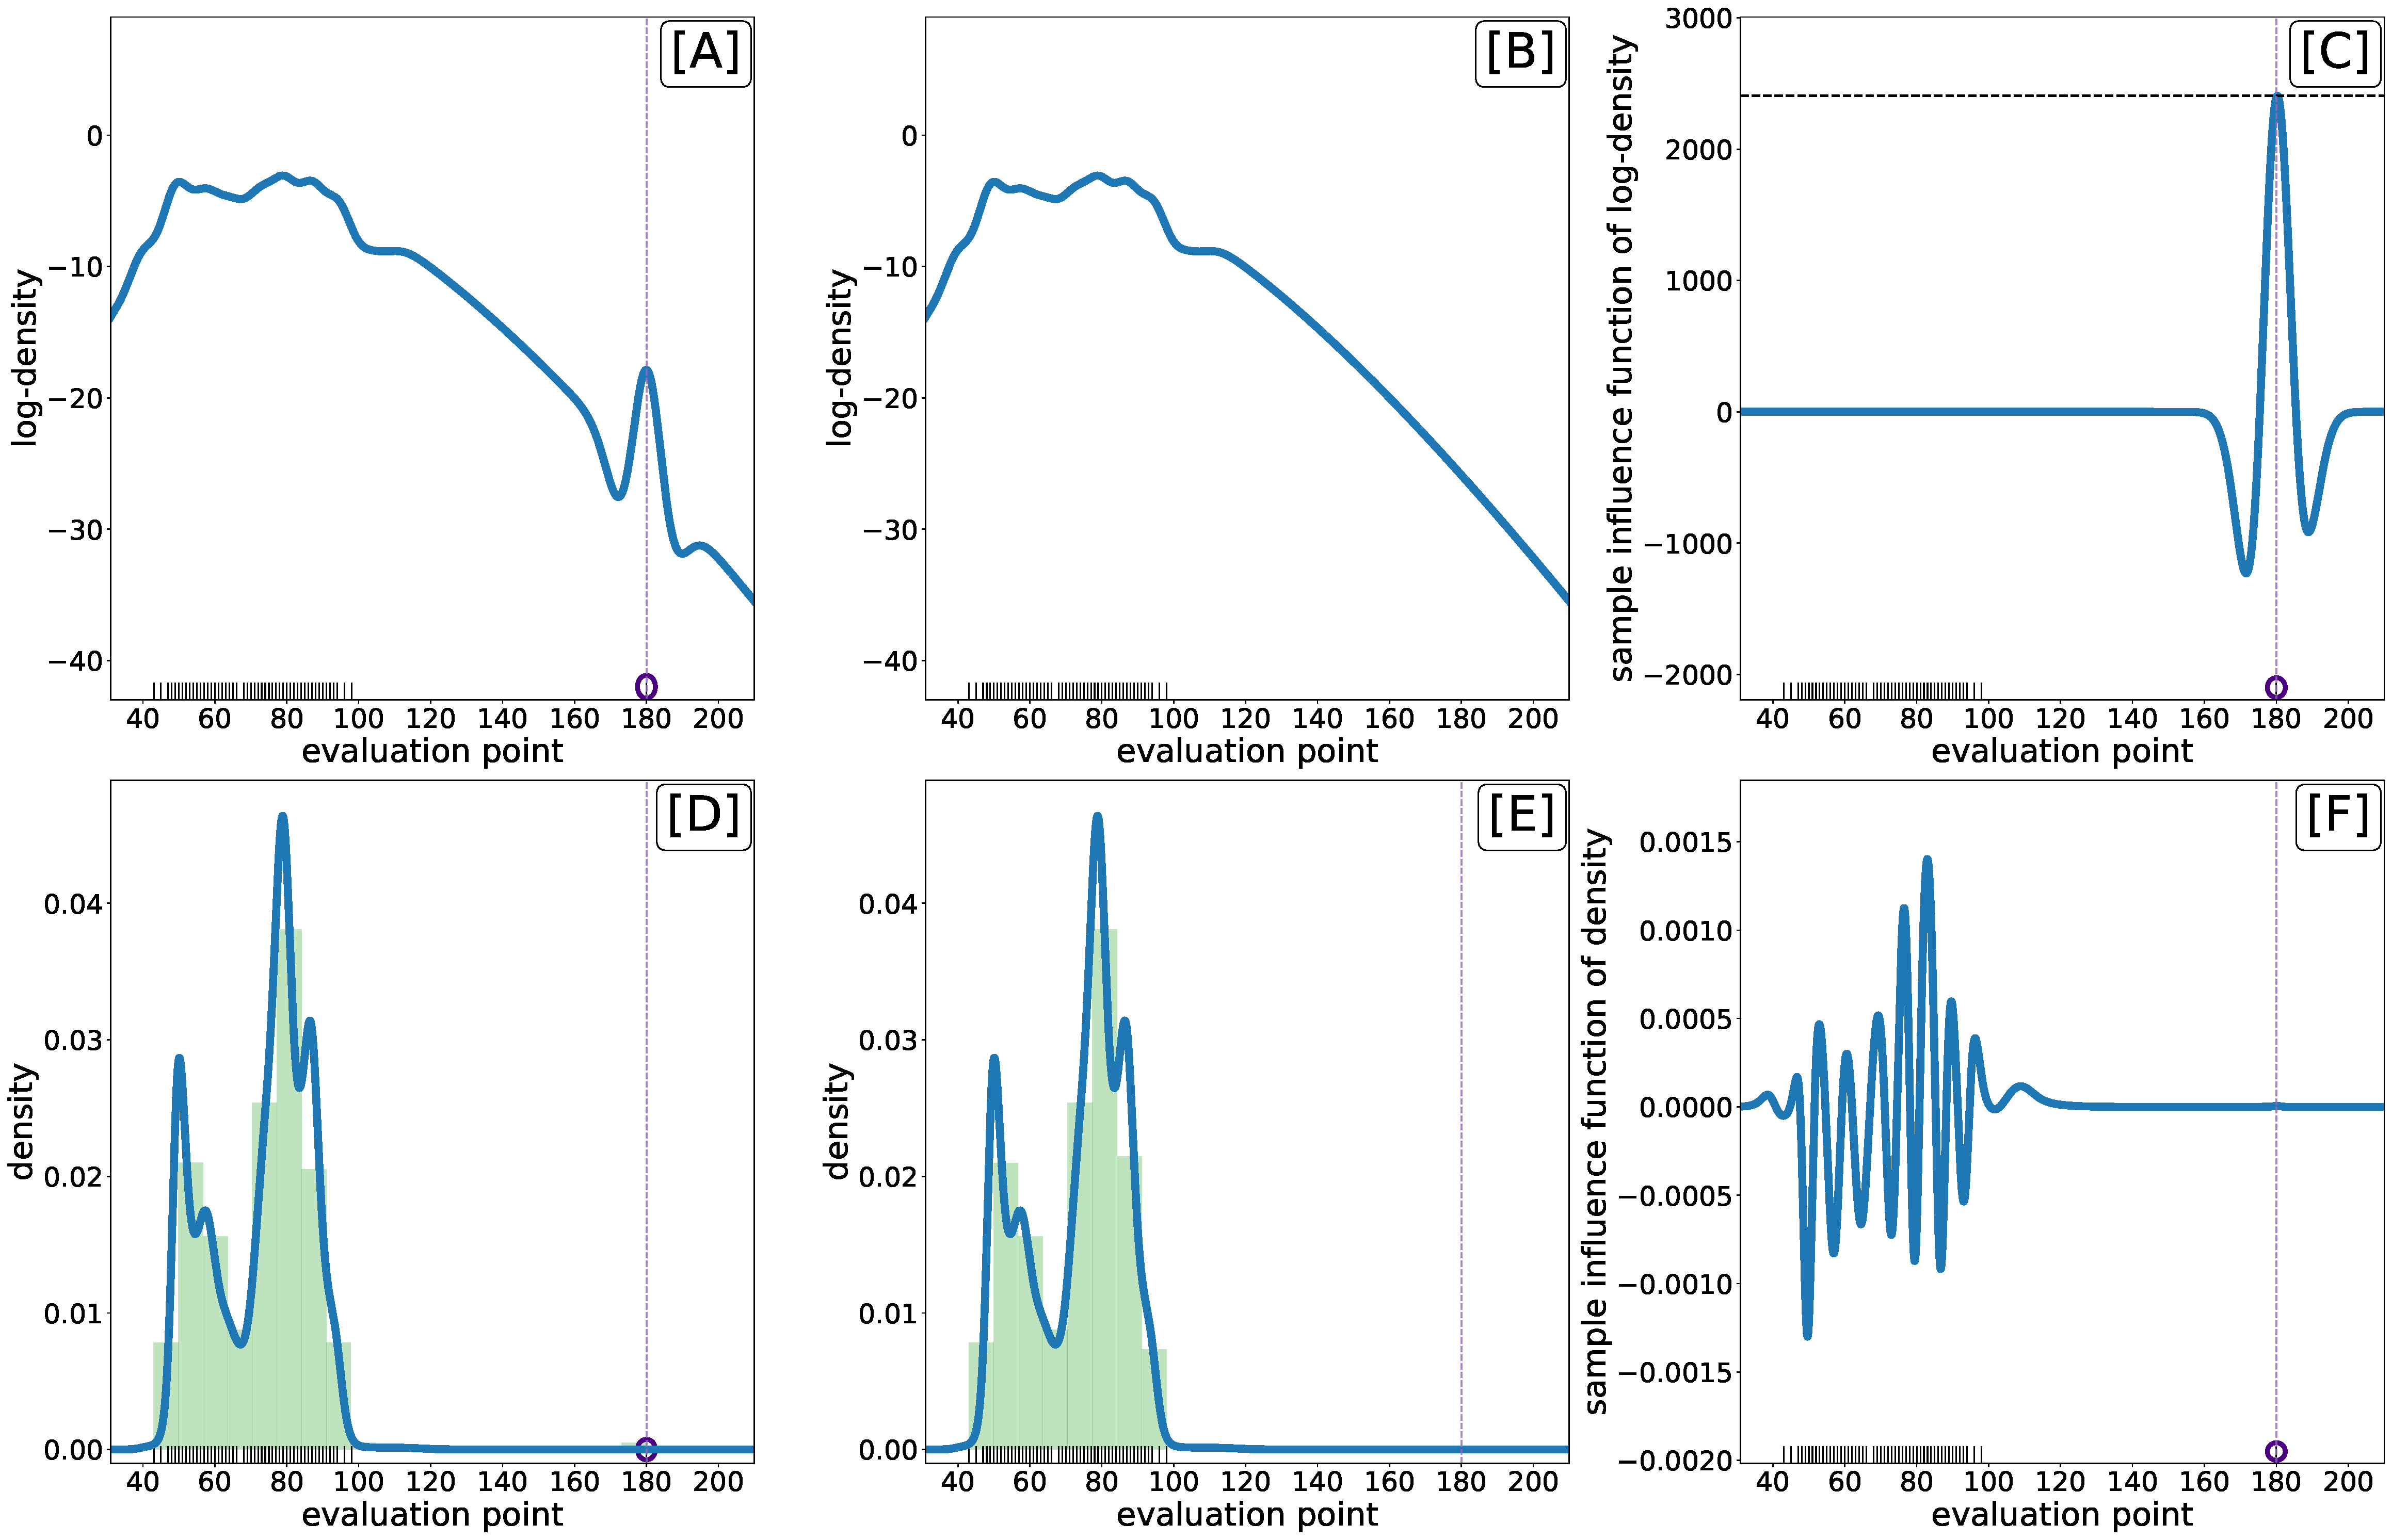
\includegraphics[width=\textwidth]{../plots/comparison-inffunden-inffunlogden-logdensity-density-contam-sm-logpenparam=-11.0-data=180.0-gamma-36.0-2.0.pdf}
	\caption{Fix $\rho = e^{-11}$. Panels [A] and [B] show the penalized SM log-density estimates with and without the additional observation $y = 180$, respectively. Panel [C] shows the sample influence function of the log-density estimator. Panels [D] and [E] show the penalized SM density estimates with and without the additional observation $y = 180$, respectively. Panel [F] shows the resulting sample influence function of the density estimator. The rug plot indicates the location of data and the purple circle indicates the location of the observation $y=180$.}
	\label{fig-inffun-logdensity-vs-density-sm-y=180}
\end{figure}

\begin{figure}% [h!]
	\centering 
	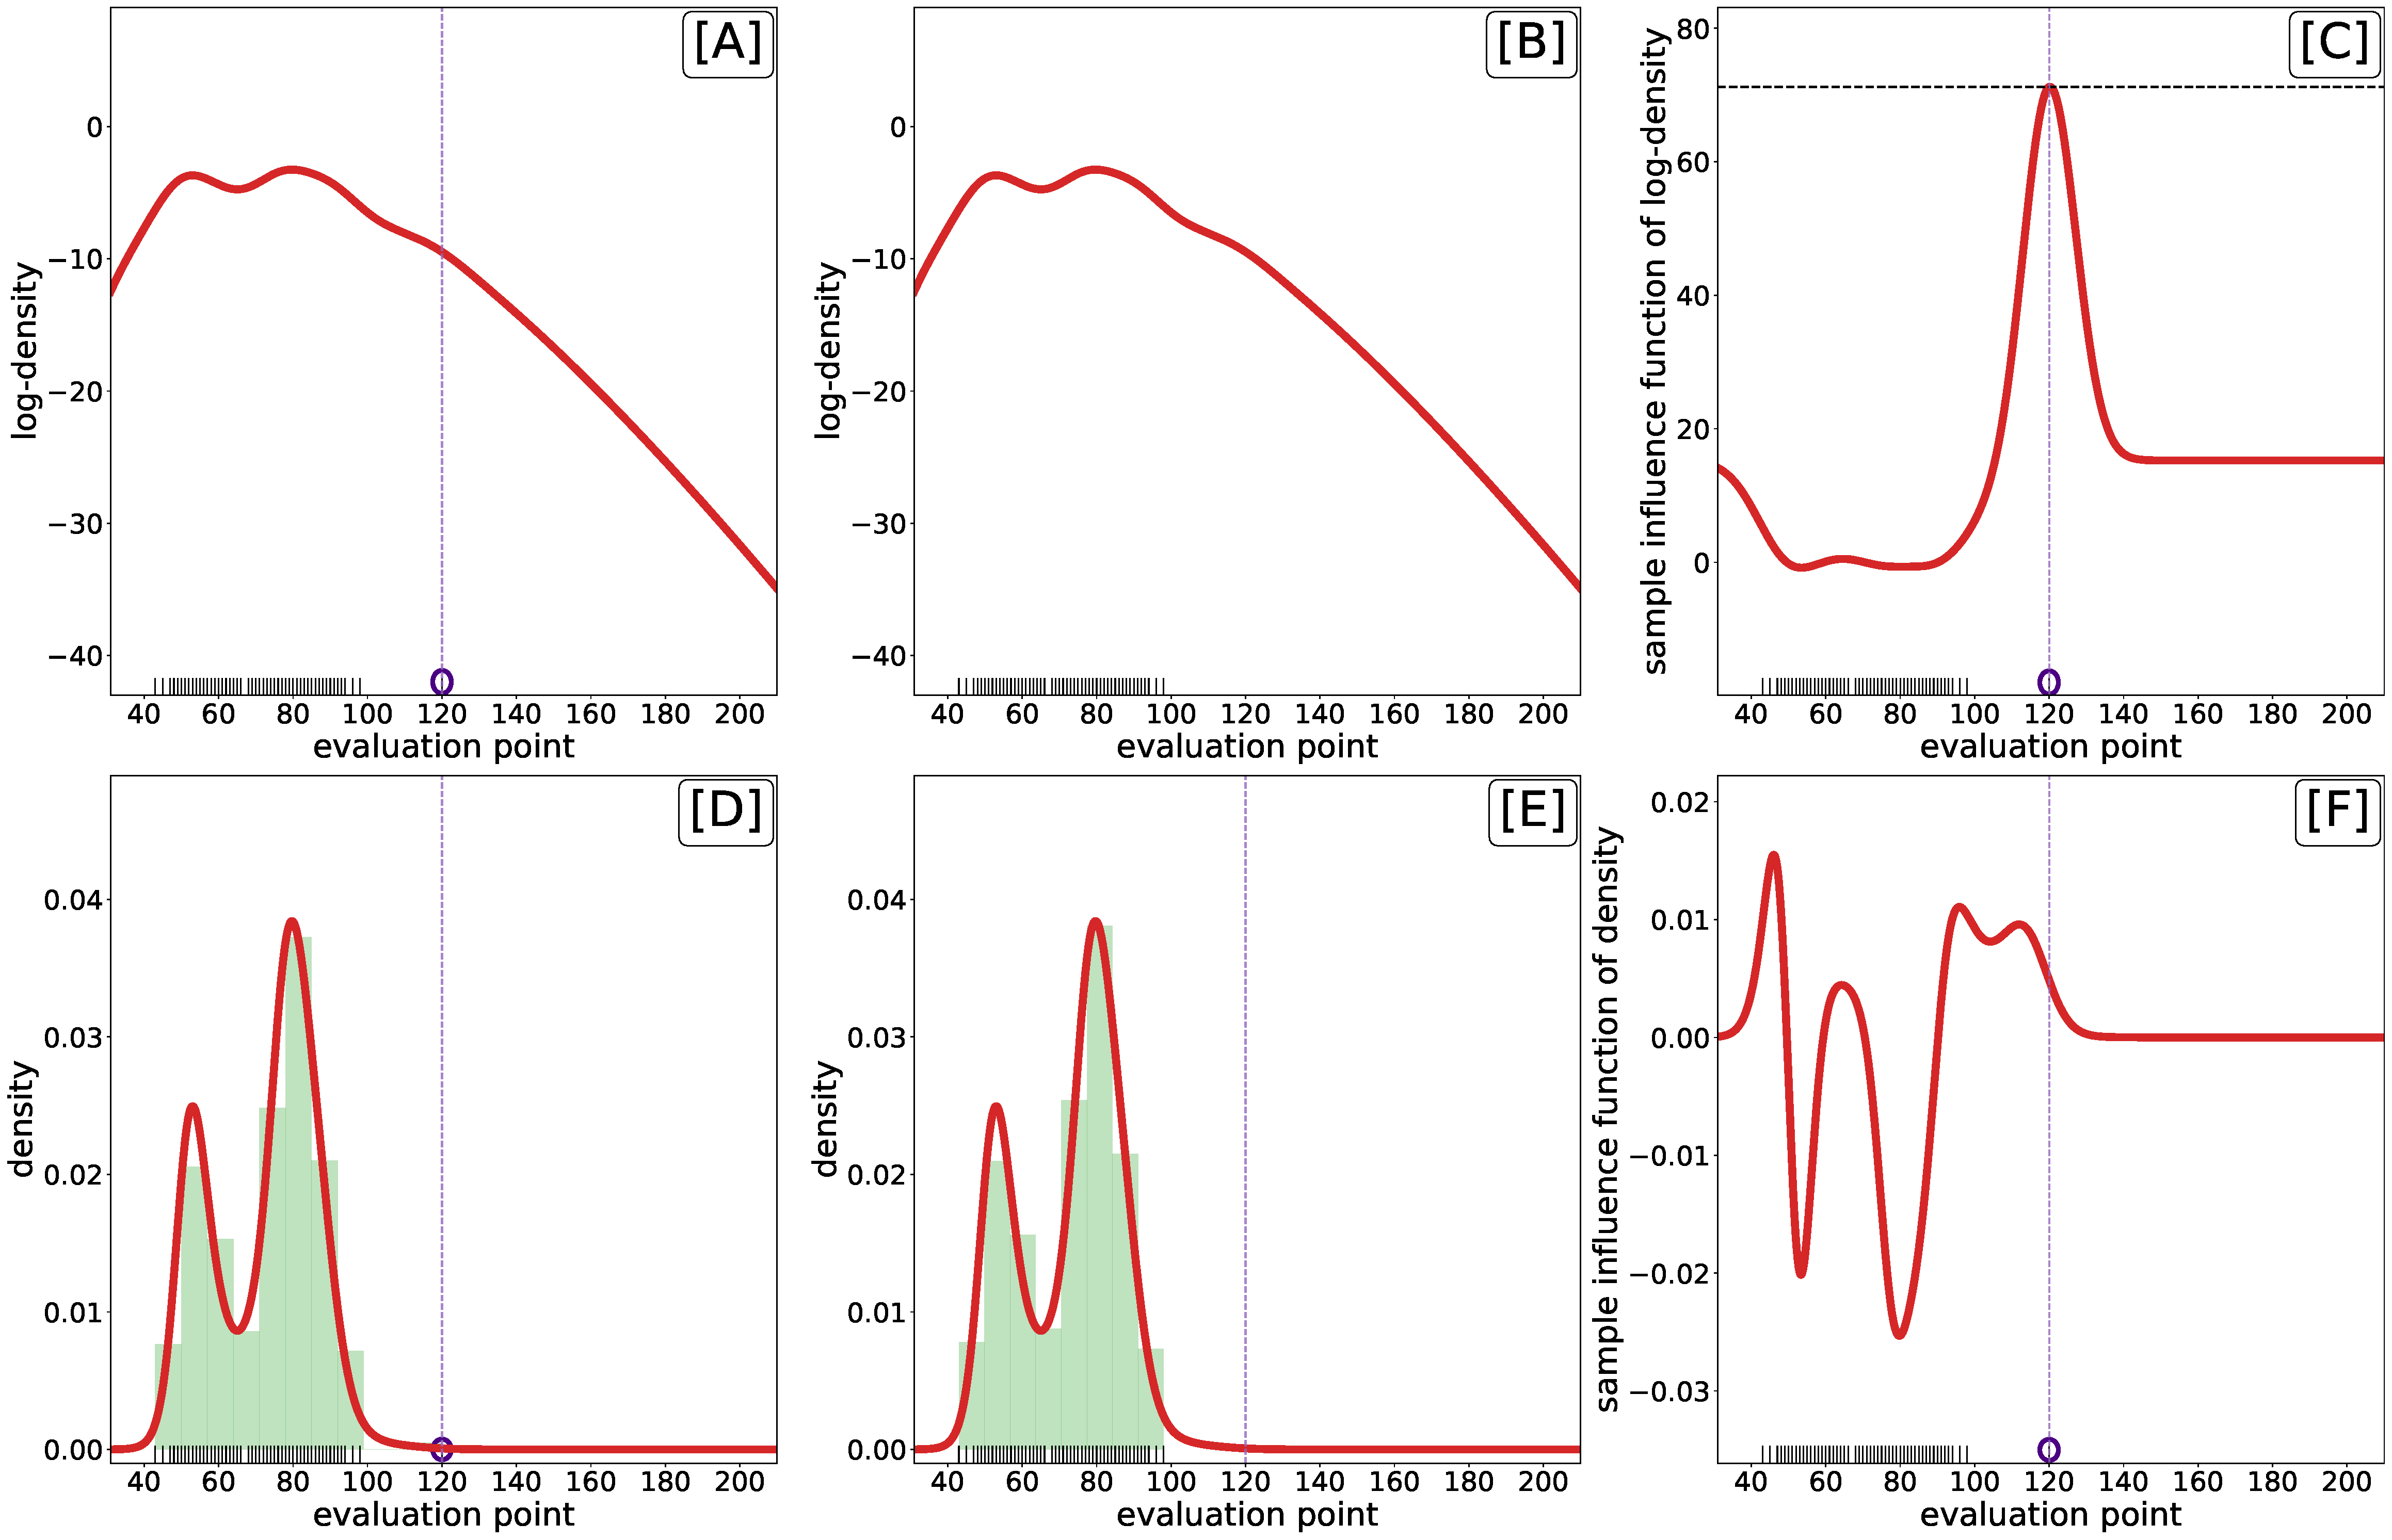
\includegraphics[width=\textwidth]{../plots/comparison-inffunden-inffunlogden-logdensity-density-contam-ml-logpenparam=-15.0-data=120.0-gamma-36.0-2.0.pdf}
	\caption{Fix $\lambda = e^{-15}$. Panels [A] and [B] show the penalized ML log-density estimates with and without the additional observation $y = 120$, respectively. Panel [C] shows the sample influence function of the log-density estimator. Panels [D] and [E] show the penalized SM density estimates with and without the additional observation $y = 120$, respectively. Panel [F] shows the resulting sample influence function of the density estimator. The rug plot indicates the location of data and the purple circle indicates the location of the observation $y=120$.}
	\label{fig-inffun-logdensity-vs-density-ml-y=120}
\end{figure}

\begin{figure}% [h!]
	\centering 
	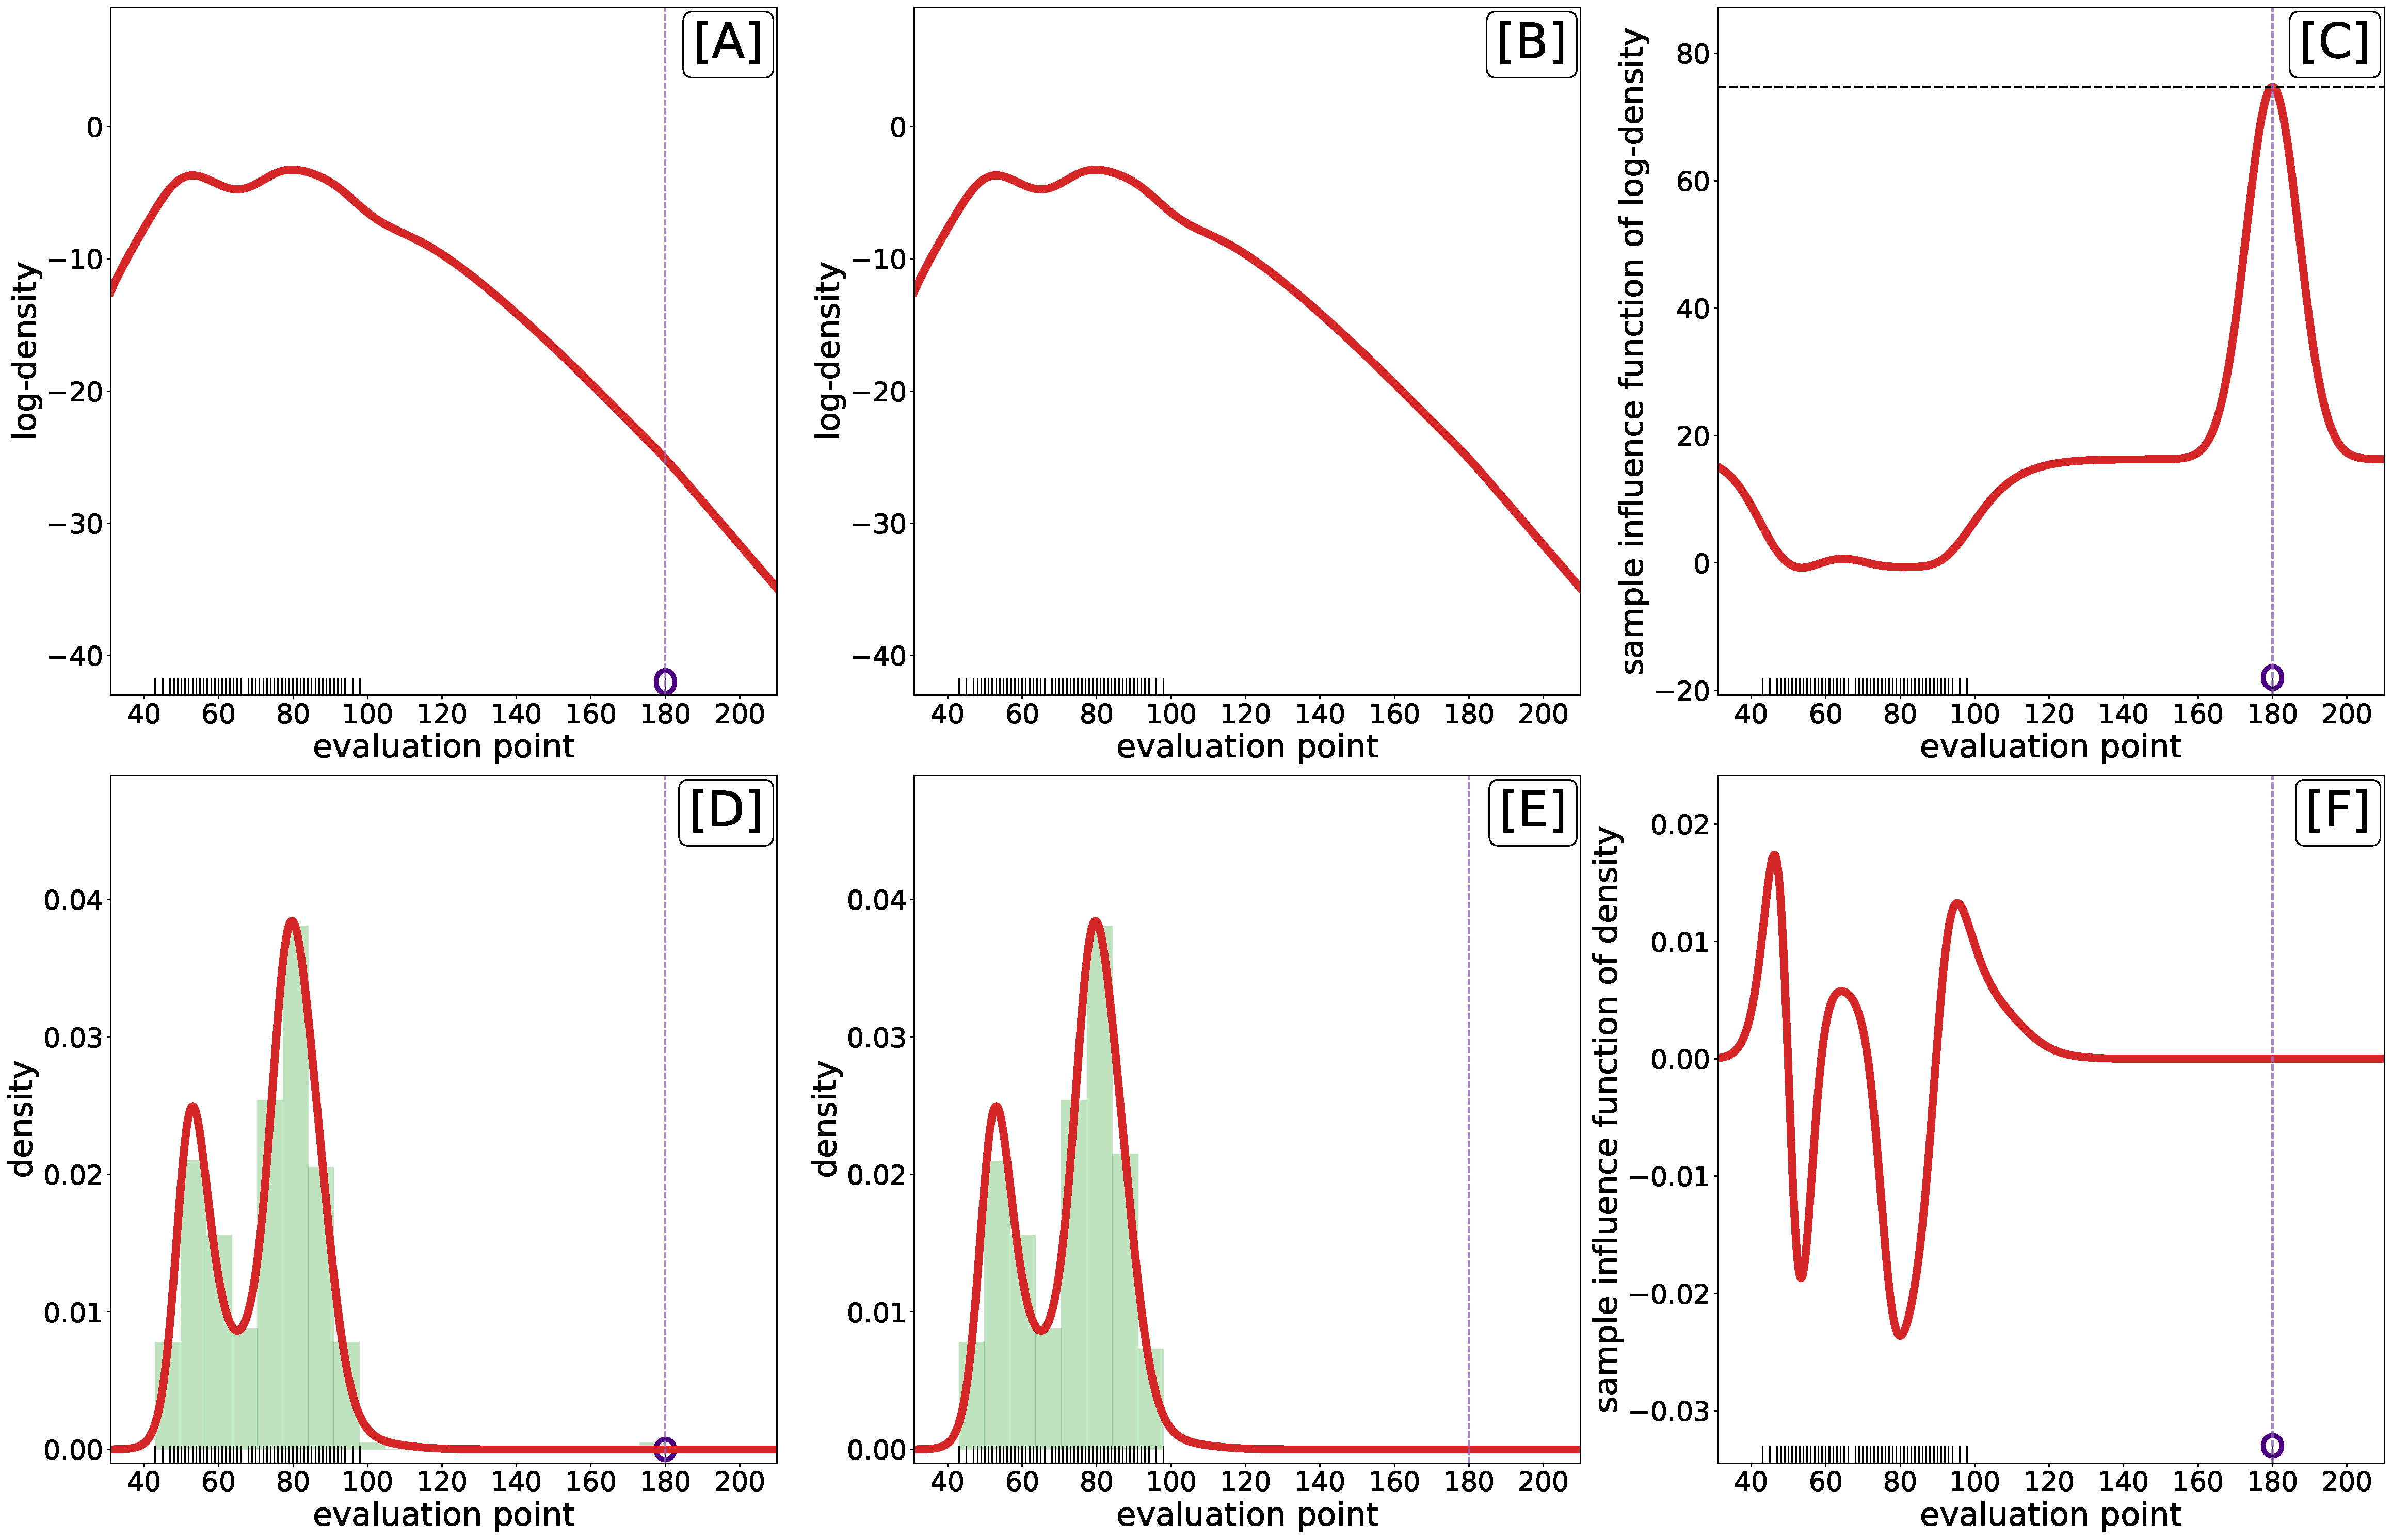
\includegraphics[width=\textwidth]{../plots/comparison-inffunden-inffunlogden-logdensity-density-contam-ml-logpenparam=-15.0-data=180.0-gamma-36.0-2.0.pdf}
	\caption{Fix $\lambda = e^{-15}$. Panels [A] and [B] show the penalized ML log-density estimates with and without the additional observation $y = 180$, respectively. Panel [C] shows the sample influence function of the log-density estimator. Panels [D] and [E] show the penalized SM density estimates with and without the additional observation $y = 180$, respectively. Panel [F] shows the resulting sample influence function of the density estimator. The rug plot indicates the location of data and the purple circle indicates the location of the observation $y=180$.}
	\label{fig-inffun-logdensity-vs-density-ml-y=180}
\end{figure}

Analytically, note that 
\begin{align*}
	& \, S_{\rho} \parens{ \parens{1 - \varepsilon_0} F_n + \varepsilon_0 \delta_y } \parens{x} - S_{\rho} \parens{F_n} \parens{x} \\ 
	= & \, \bracks[\big]{ \cancel{\log \mu \parens{x}} + f_{\SM, \parens{1 - \varepsilon_0} F_n + \varepsilon_0 \delta_y}^{\parens{\rho}} \parens{x} - A \parens{f_{\SM, \parens{1 - \varepsilon_0} F_n + \varepsilon_0 \delta_y}^{\parens{\rho}} } } \\ 
	& \qquad \quad - \bracks[\big]{ \cancel{\log \mu \parens{x}} + f_{\SM, F_n}^{\parens{\rho}} \parens{x} - A \parens{f_{\SM, F_n}^{\parens{\rho}} } } \\
	= & \, \bracks[\big]{ f_{\SM, \parens{1 - \varepsilon_0} F_n + \varepsilon_0 \delta_y}^{\parens{\rho}} \parens{x} - A \parens{f_{\SM, \parens{1 - \varepsilon_0} F_n + \varepsilon_0 \delta_y}^{\parens{\rho}} } } - \bracks[\big]{ f_{\SM, F_n}^{\parens{\rho}} \parens{x} - A \parens{f_{\SM, F_n}^{\parens{\rho}} } }, 
\end{align*}
from which we see $\mathrm{SIF}_{x, \varepsilon_0} \parens{S_{\rho}, F, y}$ does \textit{not} depend on $\mu \parens{x}$, but only on the natural parameter part. If we work with $\mathrm{SIF}_{x, \varepsilon_0} \parens{\widetilde{S}_{\rho}, F, y}$, however, we have 
\begin{align*}
	& \, \widetilde{S}_{\rho} \parens{ \parens{1 - \varepsilon_0} F_n + \varepsilon_0 \delta_y } \parens{x} - \widetilde{S}_{\rho} \parens{F_n} \parens{x} \\ 
	= & \, \mu \parens{x} \bracks[\Big]{\exp \parens[\big]{f_{\SM, \parens{1 - \varepsilon_0} F_n + \varepsilon_0 \delta_y}^{\parens{\rho}} \parens{x} - A \parens{f_{ \SM, \parens{1 - \varepsilon_0} F_n + \varepsilon_0 \delta_y}^{\parens{\rho}}}} - \exp \parens[\big]{f_{\SM, F_n}^{\parens{\rho}} \parens{x} - A \parens{f_{\SM, F_n }^{\parens{\rho}}}} }, 
\end{align*}
and we cannot get rid of $\mu \parens{x}$ in the front. The resulting $\mathrm{SIF}_{x, \varepsilon_0} \parens{\widetilde{S}_{\rho}, F, y}$ inevitably depends on $\mu \parens{x}$. By a similar approach as above, we can also see $\mathrm{SIF}_{x, \varepsilon_0} \parens{T_{\lambda}, F, y}$ does \textit{not} depend on $\mu \parens{x}$ but $\mathrm{SIF}_{x, \varepsilon_0} \parens{\widetilde{T}_{\lambda}, F, y}$ does. 

Thus, from both numerical examples and analytic analysis, we see the sample influence function of the \emph{log-}density estimator is the better choice than that of the density estimator. Hence, we will only consider the former in the sequel. 


\subsection{Comparison of the Sensitivities}\label{subsection-main-comparison-sensitivity}

Our goal of this section is to compare the sensitivities of the penalized ML and SM density estimators in $\calQ_{\ker}$. 

Let us still fix $\rho = e^{-11}$ and $y = 120$, and return to the first row of Figure \ref{fig-inffun-logdensity-vs-density-sm-y=120} where we show $S_{\rho} \parens{\parens{1 - \varepsilon_0} F_n + \varepsilon_0 \delta_y}$, $S_{\rho} \parens{F_n}$, and the resulting sample influence function evaluated at different points. It is apparent that $y = 120$ has different effects on $S_{\rho}$ at different evaluation points. The overall influence of $y$ on $S_{\rho}$, $\widehat{M}_{\varepsilon_0} \parens{S_{\rho}, F_n, y}$, is approximately equal to 2315.48, which is achieved roughly at 120. 

Let us still fix $\rho = e^{-11}$ but vary $y$. The left panel in Figure \ref{fig-SM-overall} shows the overall influence of $y$ on $S_{\rho}$ against different choices of $y$. It is obvious that different locations of $y$ have different overall influences on $S_{\rho}$. When $y$ is below 40 or above 100 (low-density region), it has a larger overall influence on $S_{\rho}$; and when $y$ is between 40 and 100 (high-density region), it has a smaller overall influence. 

\begin{figure}[h]
	\centering
	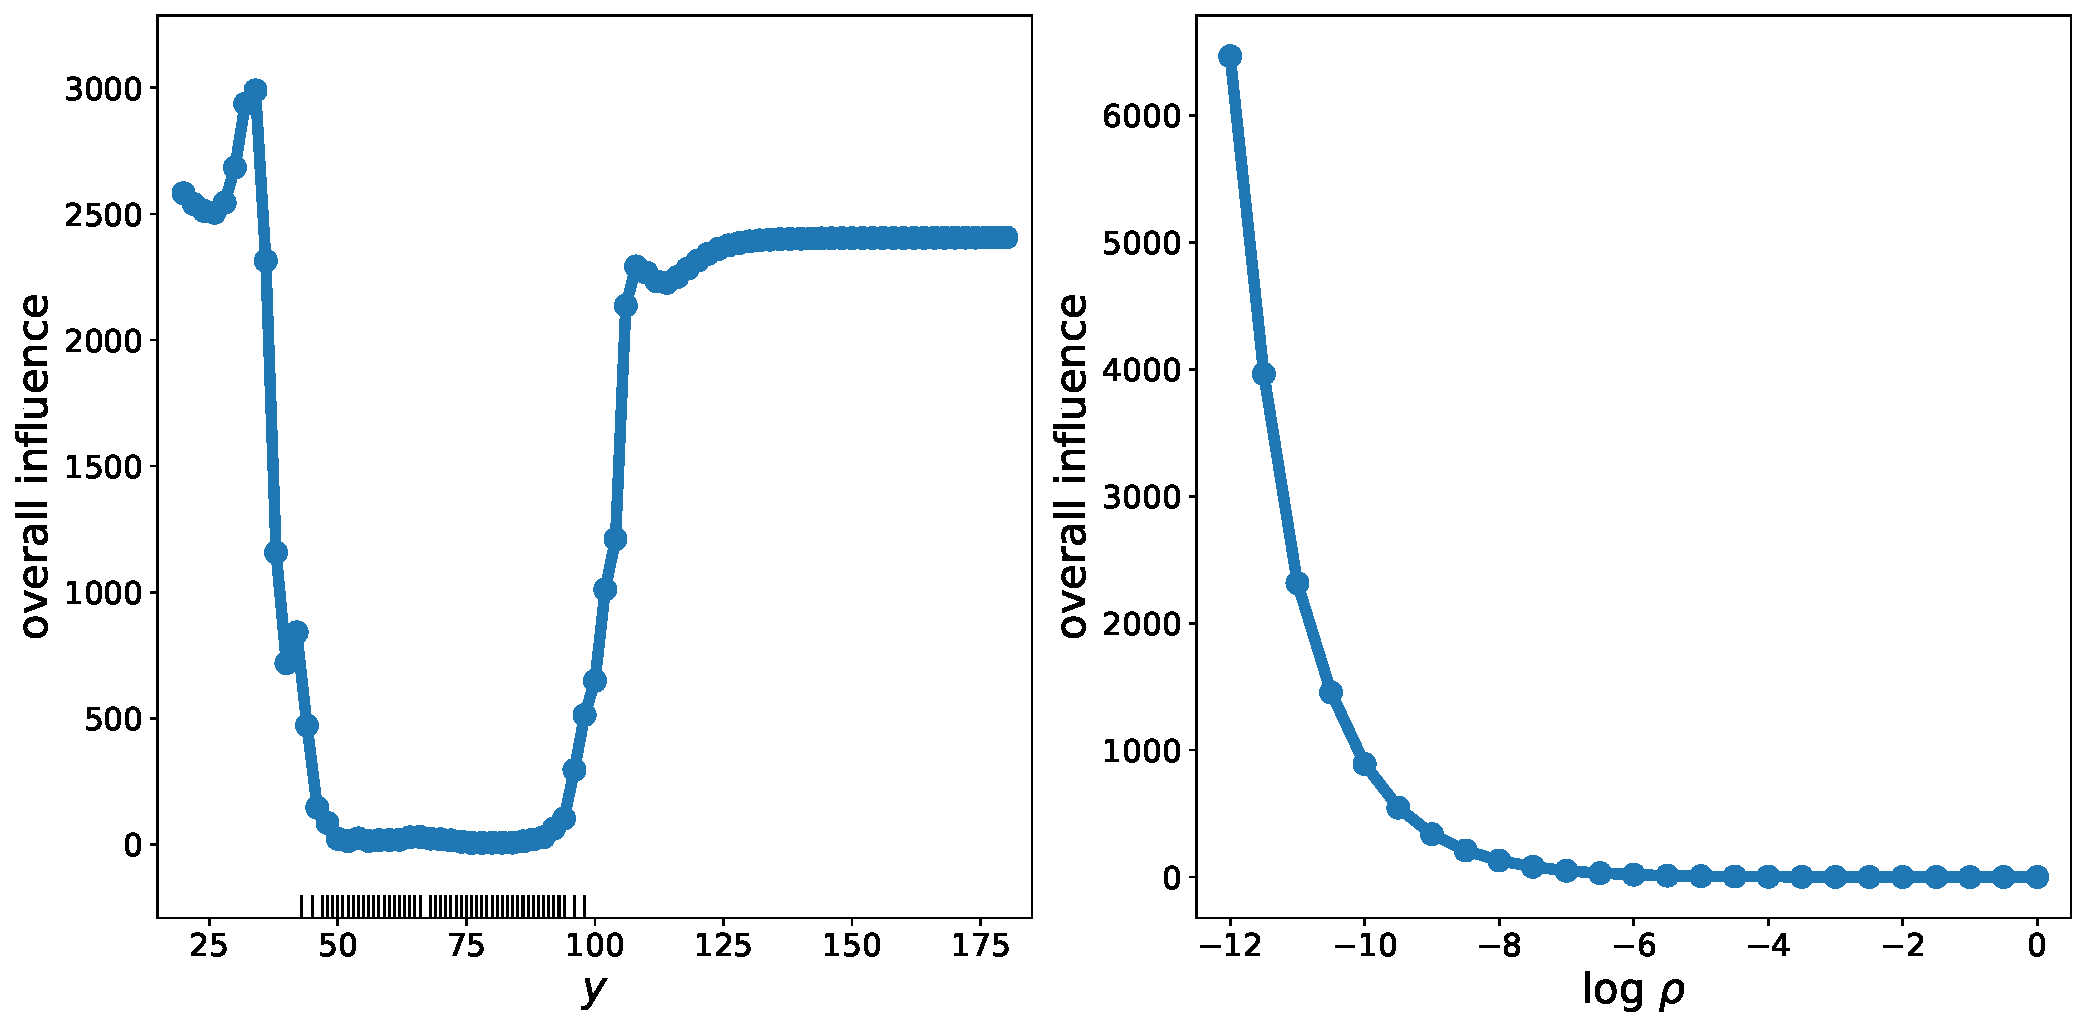
\includegraphics[width=\textwidth]{../plots/waiting-SM-overall-empirical-influence-log-density-estimates-baseden=Gamma-36-2-gridpoints=1-202-1.pdf}
	\caption{Left panel shows the overall influence versus different choices of $y$, where we fix $\rho = e^{-11}$ and the rug plot indicate the location of the \texttt{waiting} data. Right panel shows the overall influence against different choices of $\rho$ (shown in log scale), where we fix $y = 120$.}
	\label{fig-SM-overall}
\end{figure}

Now, fix $y = 120$ but vary the values of $\rho$. The right panel in Figure \ref{fig-SM-overall} shows the overall influence of $y = 120$ on $S_{\rho}$ versus different choices of $\rho$. It is obvious that the overall influence of $y$ keeps increasing as the value of $\rho$ keeps decreasing. 

Thus, both the location of $y$ and the value of $\rho$ impact the overall influence on log-density estimators. To exhibit the sensitivity of the penalized SM log-density estimators subject to these two factors, a natural idea is to plot the heat map of the overall influence against them, which is shown in Figure \ref{fig-SM-overall-influence-y-rho}. However, recall our ultimate goal is to compare the sensitivities of both penalized ML and SM density estimators, and their respective penalty parameters, $\lambda$ and $\rho$, are on different scales. Thus, plotting the penalty parameter on the horizontal axis is not conducive to comparison. Instead, we plot the RKHS norm of natural parameter under $F_n$, i.e., $\norm{f_{\ML, F_n}^{\parens{\lambda}}}_{\calH}$ and $\norm{f_{\SM, F_n}^{\parens{\rho}}}_{\calH}$, on the horizontal axis. The smaller the penalty parameter is, the larger the RKHS norm of the natural parameter is. 

\begin{figure}[h]
	\centering
	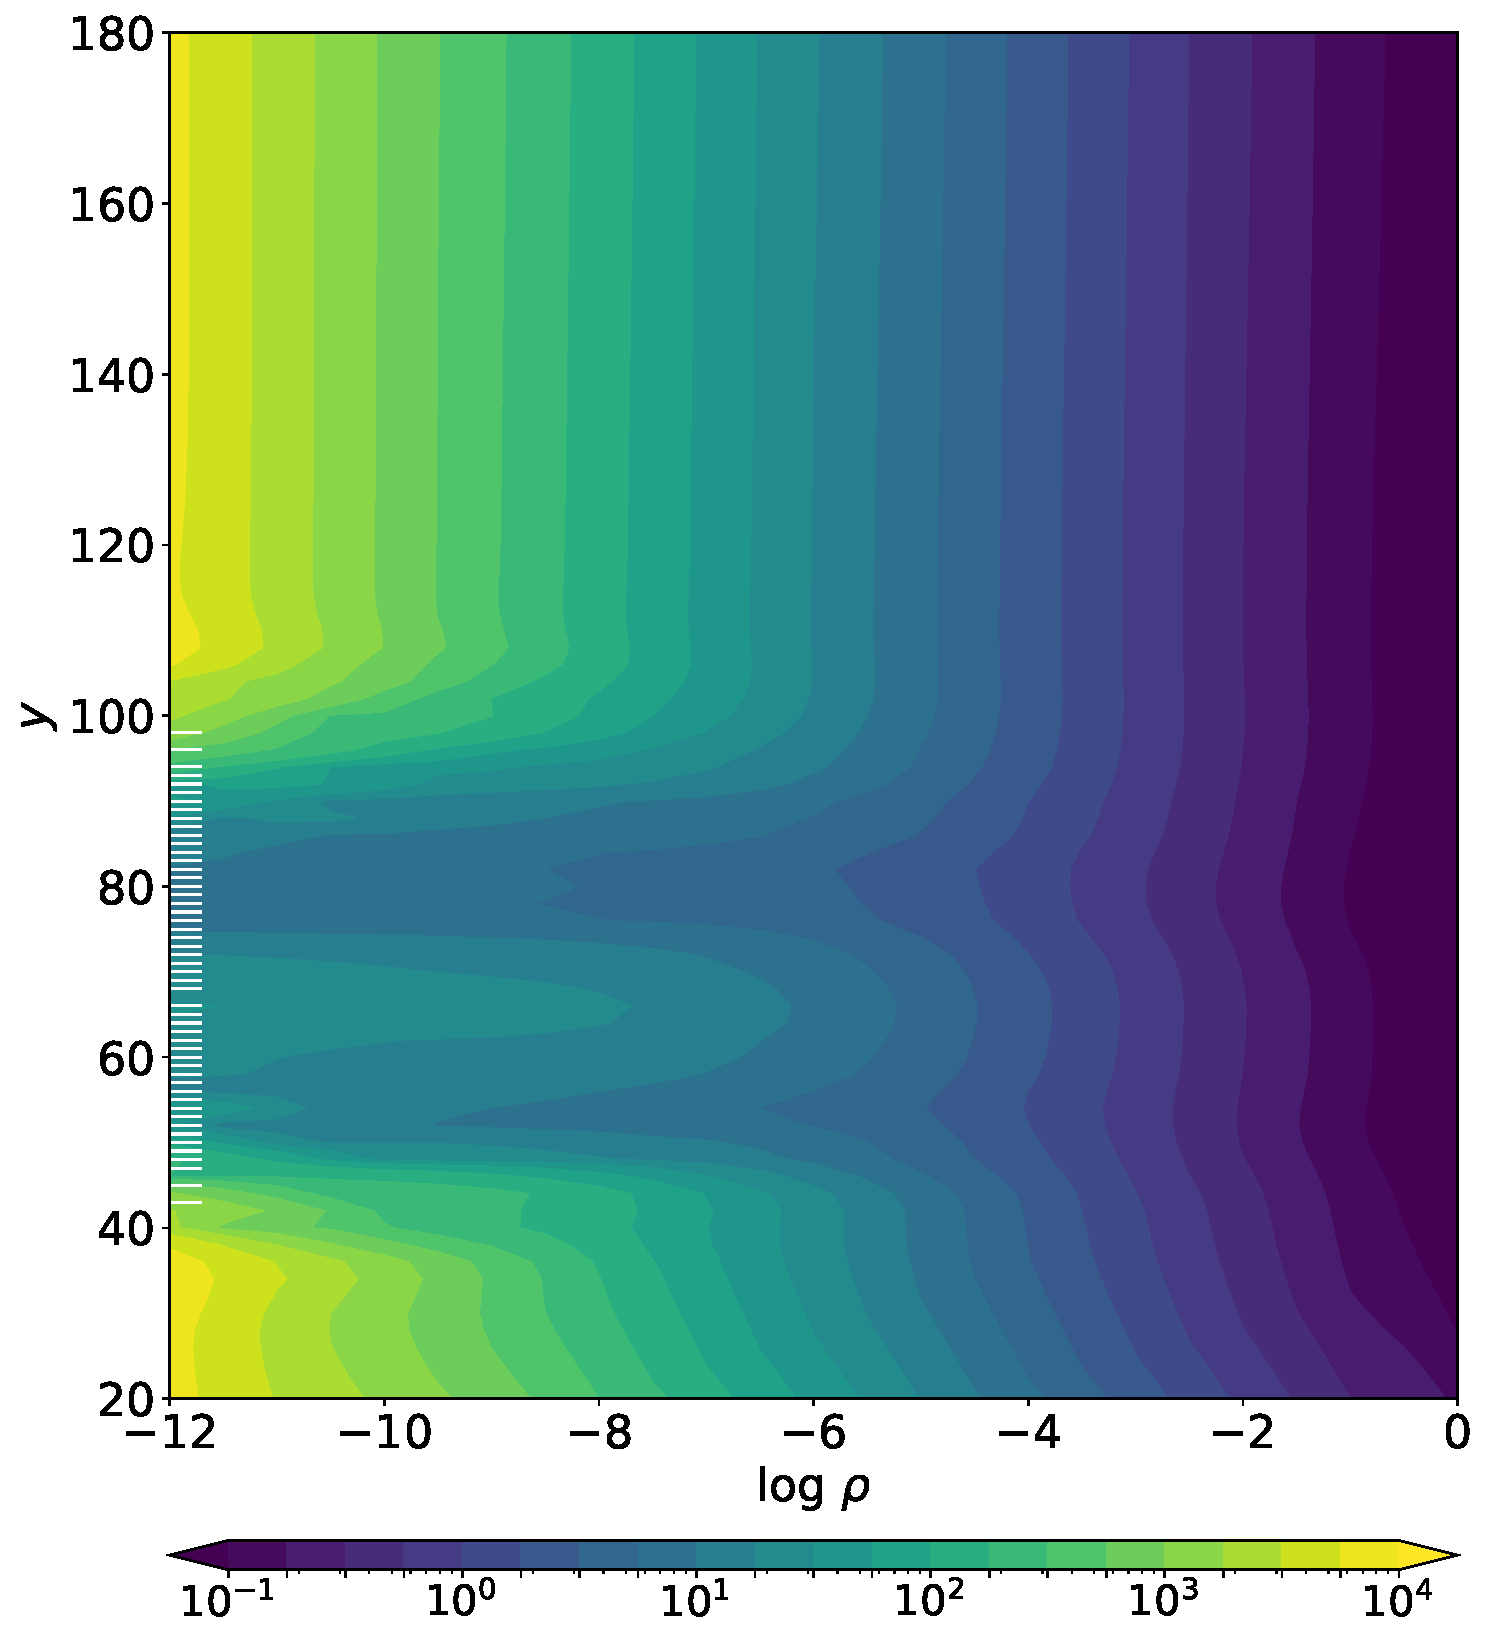
\includegraphics[width=0.6\textwidth]{../plots/PenSMFin-PenML-geyser-waiting-logdensity-empIF-supnorm-penaltyparameter-heatmap-bw=5.0-Gamma-36-2-gridpoints=1-202-1-logscale.pdf}
	\caption{Heat map of the overall influence on the penalized SM log-density estimates against $y$ and $\rho$ (shown in log scale). White rugs indicate locations of the \texttt{waiting} data.} 
	\label{fig-SM-overall-influence-y-rho}
\end{figure}

\begin{figure}[h!]
	\centering
	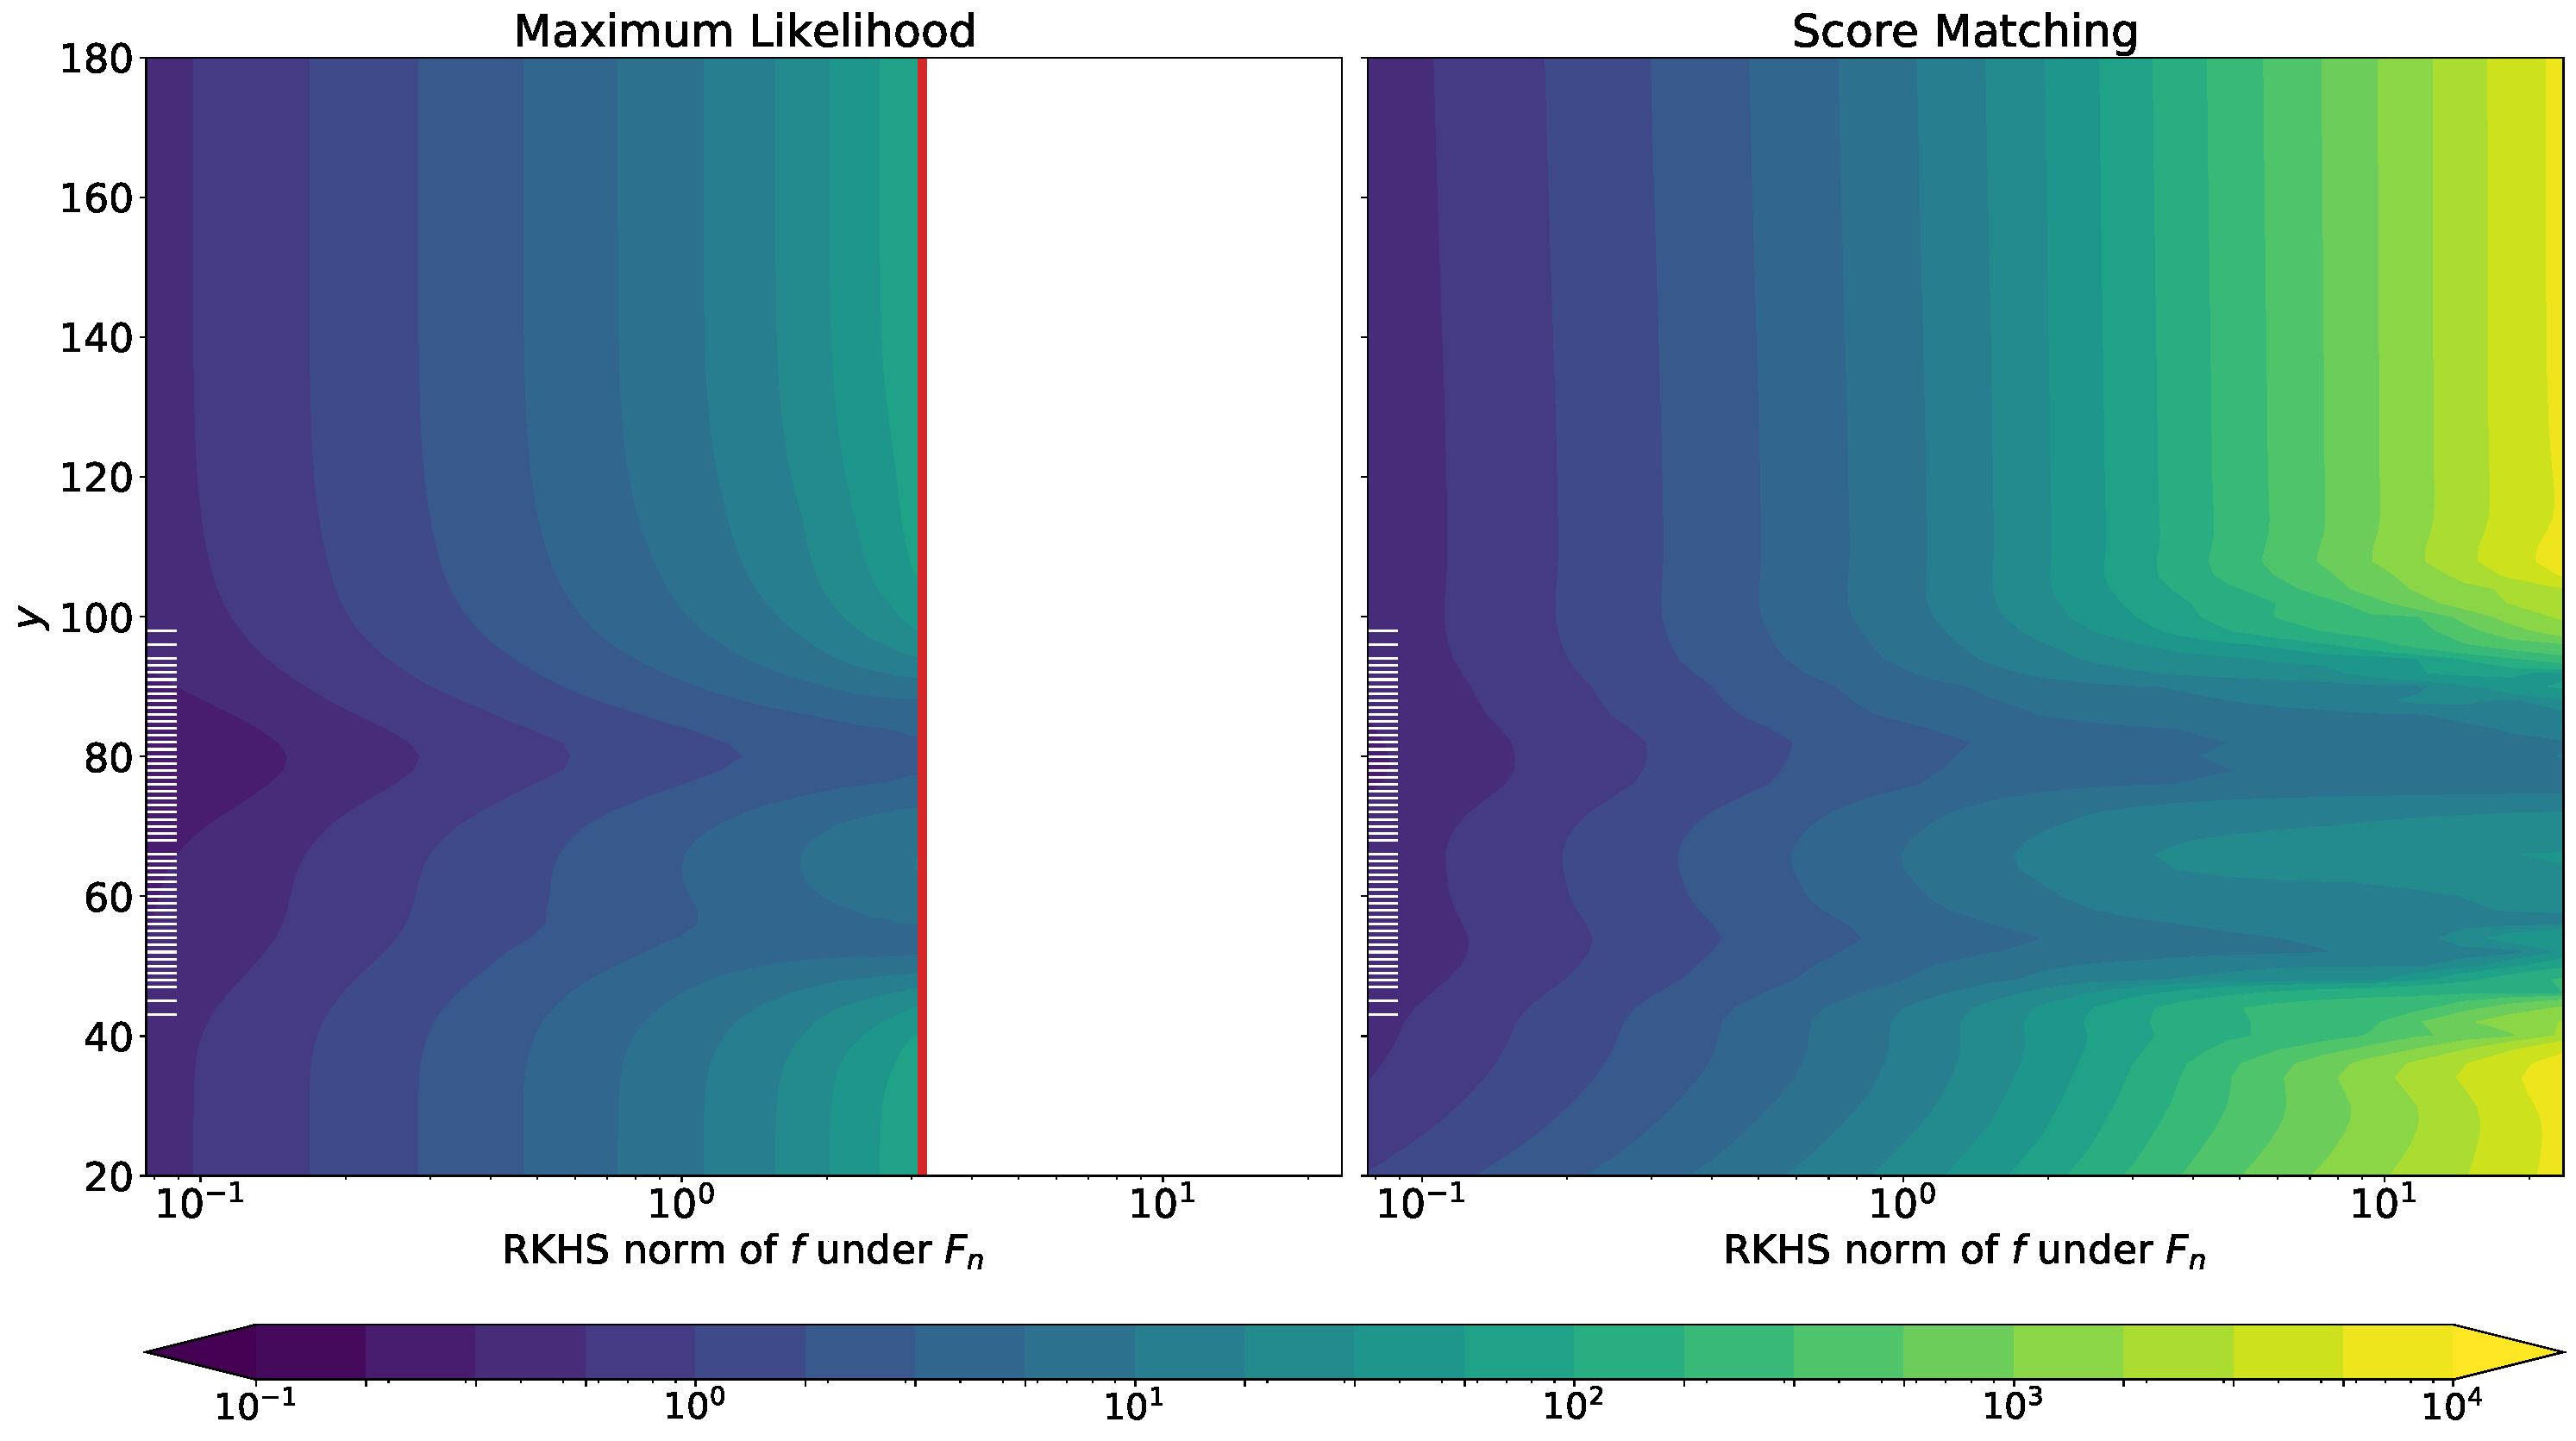
\includegraphics[width=\textwidth]{../plots/PenSMFin-PenML-geyser-waiting-logdensity-empIF-supnorm-natparamnorm-heatmap-bw=5.0-Gamma-36-2-gridpoints=1-202-1-logscale.pdf}
	\caption{Heat maps of the overall influence on penalized ML (left) and SM (right) log-density estimates against $y$ and the RKHS norm of the natural parameter under $F_n$ (shown in log scale). Red vertical line in left panel indicates the case $\lambda = 0$. White rugs indicate locations of the \texttt{waiting} data.}
	\label{fig-SM-overall-influence-y-norm}
\end{figure}

The resulting heat maps for the penalized ML and SM density estimates are shown in Figure \ref{fig-SM-overall-influence-y-norm}, where we choose $y = 20, 22, \cdots, 180$, $\lambda = 0, e^{-15}, e^{-14.5}, \cdots, e^{0.5}, e^{1}$, and $\rho = e^{-12}, e^{-11.5}, \cdots, e^{0}$. If we look at each panel individually, findings are consistent as before: with a fixed value of the penalty parameter, $y$ in the low-density region has a larger overall influence on log-density estimates than that in the high-density region; with a fixed $y$, a larger RKHS norm of the natural parameter (corresponding to a smaller penalty parameter value) implies a larger overall influence of $y$. In particular, if we fix a $y$ value, say $y_0$, the maximal possible overall influence of $y_0$ on the penalized ML density estimates for all values of $\lambda \ge 0$ is the intersection of $y = y_0$ and the red vertical line, which corresponds to the overall influence of $y_0$ on the unpenalized ML density estimate (i.e., $\lambda = 0$). 

If we compare two panels in Figure \ref{fig-SM-overall-influence-y-norm}, we observe that, for each choice of $y$, as we decrease the values of penalty parameters so that the RKHS norm of $f$ under $F_n$ keeps increasing, the overall influences on the penalized ML density estimates stop increasing at the red vertical line, but that on the penalized SM density estimates can continue increasing. In other words, for each choice of $y$, the overall influences on the penalized SM log-density estimates with sufficiently small values of $\rho > 0$ are larger than the overall influence on the \emph{unpenalized} ML log-density estimate, implying that, when there is a small amount of penalization, the penalized SM density estimator is more sensitive to an additional observation (not only to the isolated observation) than the unpenalized and penalized ML density estimator. Additional numerical examples also confirm our observations here. 


\section{The Sensitivity of $K$-fold Cross-validated Penalized Score Matching Density Estimator}\label{section-sensitivity-cv-penalized-sm-density-estimator}

$K$-fold cross-validation (CV) is perhaps the most popular method to choose the penalty parameter in practice. In this section, we are going to investigate whether the $K$-fold cross-validated penalized SM density estimator is sensitive to the presence of an additional observation or not. The procedure of computing the overall influence of $y$ on the $K$-fold cross-validated penalized SM density estimator is shown in Algorithm \ref{algo-sensitivity-cv-sm-density-estimator}. 

\begin{algorithm}
\caption{Computation of the overall influence of $K$-fold cross-validated penalized SM density estimator}\label{algo-sensitivity-cv-sm-density-estimator}
\begin{algorithmic}[1]
\Statex \algorithmicrequire 
\begin{itemize}\setlength\itemsep{0em}
	\item $X_1, \cdots, X_n$, data; 
	\item $y \in \calX$, contaminant; 
	\item $K$, the number of folds in CV; 
	\item $\sets{\rho_j}_{j=1}^{M}$, a list of penalty parameter candidates; 
	\item $\widetilde{\calH}$, the finite-dimensional approximating subspace over which we minimize the penalized NLL loss functional; 
	\item $\sets{x_{\ell}}_{\ell=1}^L \subset \calX$, a set of dense evaluation points in $\calX$. 
\end{itemize}

\vspace{5pt}

\State Compute the best density estimate using $X_1, \cdots, X_n$ with the penalty parameter selected by CV; denote the resulting log-density estimate by $S_{\mathrm{CV}} \parens{F_n}$; 
\State Compute the best density estimate using $X_1, \cdots, X_n$ and $y$ with the penalty parameter selected by CV; denoted the resulting log-density estimate by $S_{\mathrm{CV}} \parens{F_{n+1}}$; 
\State Compute 
\begin{align*}
	\mathrm{SIF}_{x_{\ell}, \varepsilon_0} \parens{S_{\mathrm{CV}}, F_n, y} := \parens[\Big]{S_{\mathrm{CV}} \parens{F_{n+1}} \parens{x_\ell} - S_{\mathrm{CV}} \parens{F_{n}} \parens{x_\ell}} \times \parens{n+1}, 
\end{align*}
for all $\ell = 1, \cdots, L$; 
\State \textbf{return} $\max_{\ell=1,\cdots,L} \abs[\big]{\mathrm{SIF}_{x_{\ell}, \varepsilon_0} \parens{S_{\mathrm{CV}}, F_n, y}}$. 
\end{algorithmic}
\end{algorithm}

We still use the \texttt{waiting} variable in the Old Faithful Geyser dataset and choose the number of folds to be $K = 3, 5, 10$. For each value of $K$, we replicate the procedures outlined in Algorithm \ref{algo-sensitivity-cv-sm-density-estimator} for 30 times. The additional observations $y$ we choose are the same as those in the preceding section, $y = 20, 22, \cdots, 180$. Figure \ref{fig-sensitivity-cv-sm-density-estimator} shows the results. 

\begin{figure}[t]
	\centering
	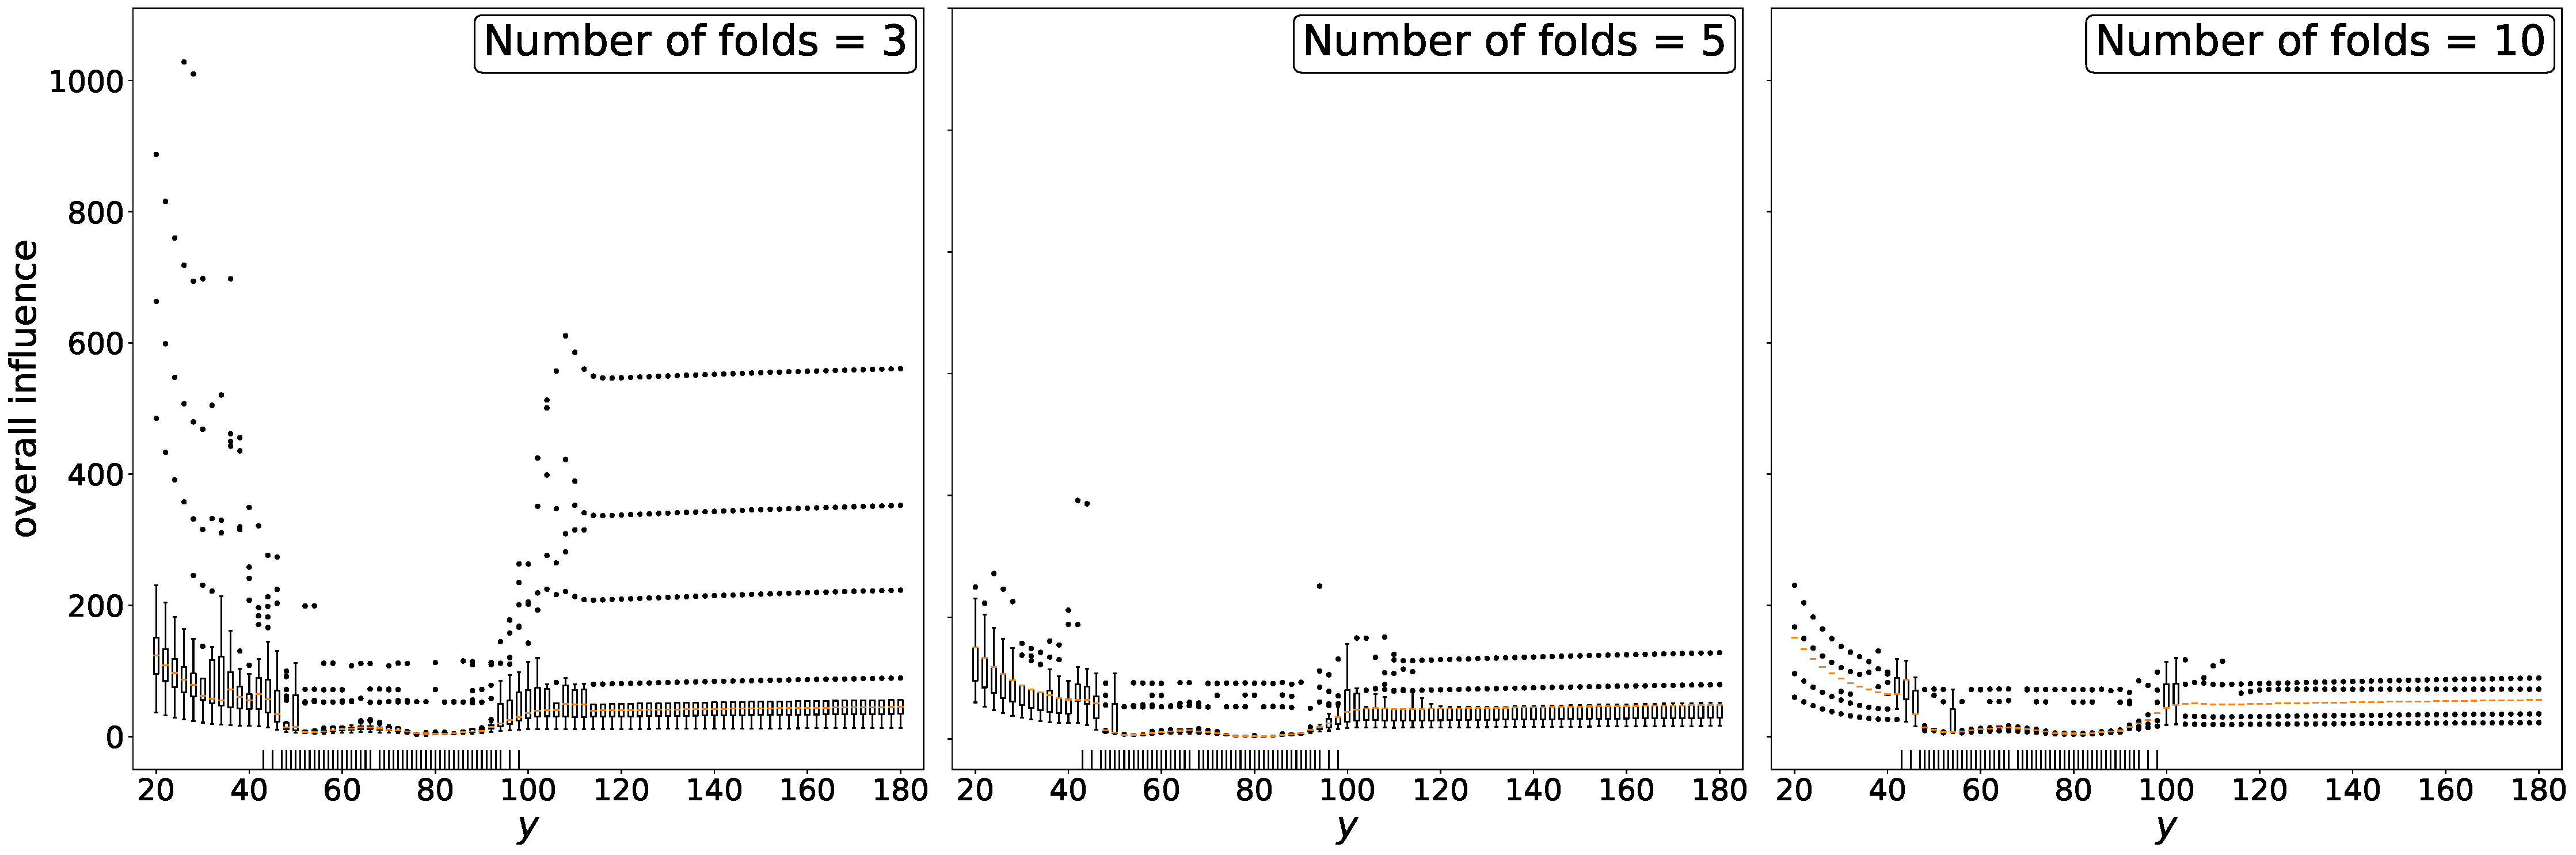
\includegraphics[width=\textwidth]{../plots/PenSMFin-geyser-waiting-overall-emp-influence-y-baseden=Gamma-36.0-2.0-gridpoints=1-202-1-cross-validation.pdf}
	\caption{Overall influence of $y$ on the $K$-fold cross-validated penalized SM density estimates against the values of $y$. We choose $K=3$ (left panel), 5 (middle panel), and 10 (right panel). In each panel, for each choice of $y$, we plot a boxplot of the overall influences of that particular $y$ value on $S_{\rho} \parens{F_n}$ obtained from 30 replications. }
	\label{fig-sensitivity-cv-sm-density-estimator}
\end{figure}

For each number of folds, similar to our earlier observations, when $y$ is in the high-density region (between 40 and 100), the overall influences of $y$ on cross-validated penalized SM density estimates tend to be small; and when $y$ is in the low-density region ($<40$ or $>100$), the overall influences of $y$ tend to be much larger. 

In addition, we see as the number of folds increases, the cross-validated penalized SM log-density estimates become less sensitive in general. %, which is mainly because, as the number of folds increases, the fraction of time that an isolated observation is included increases. 
%We see that cross-validated penalized SM log-density estimates are \emph{not} sensitive to $y$ in general, with a few exceptions when a smaller number of folds is used. 
This suggests that when one uses the $K$-fold CV to select the penalty parameter, it is better to use a relatively large number of folds, e.g., $K=5$ or $10$, in order to obtain a density estimate that is \emph{not} sensitive to the presence of an isolated observation. 


%\section{Choosing the Appropriate Penalty Parameter Using the Sensitivity}\label{section-sensitivity-choose-penalty-parameter}
%
%Our earlier discussion suggests that the sensitivity of the penalized SM density estimator is directly related to the value of the penalty parameter. This suggests that we can use the sensitivity as a tool to choose the appropriate values of the penalty parameter. 
%
%We use the \texttt{waiting} variable to illustrate the procedure. Fix $y = 120$, and let $e^{-12}, e^{-11.5}, e^{-11}, \cdots, e^{-0.5}, e^0$ be the candidates of the penalty parameter values. For each value of the penalty parameter $\rho$, we can compute $S_{\rho} \parens{F_n}$ and $S_{\rho} \parens{\parens{1 - \varepsilon_0} F_n + \varepsilon_0 \delta_y}$, using which we can obtain $\mathrm{SIF}_{x, \varepsilon_0} \parens{S_{\rho}, F_n, y}$ for different evaluation points $x \in \calX$ and the overall influence  $\widehat{M}_{\varepsilon_0} \parens{S_{\rho}, F_n, y}$. Plotting the overall influence $\widehat{M}_{\varepsilon_0} \parens{S_{\rho}, F_n, y}$ against $\log \rho$, we can obtain Figure \ref{fig-choose-appro-log-pen-param}. 
%
%\begin{figure}
%	\centering
%	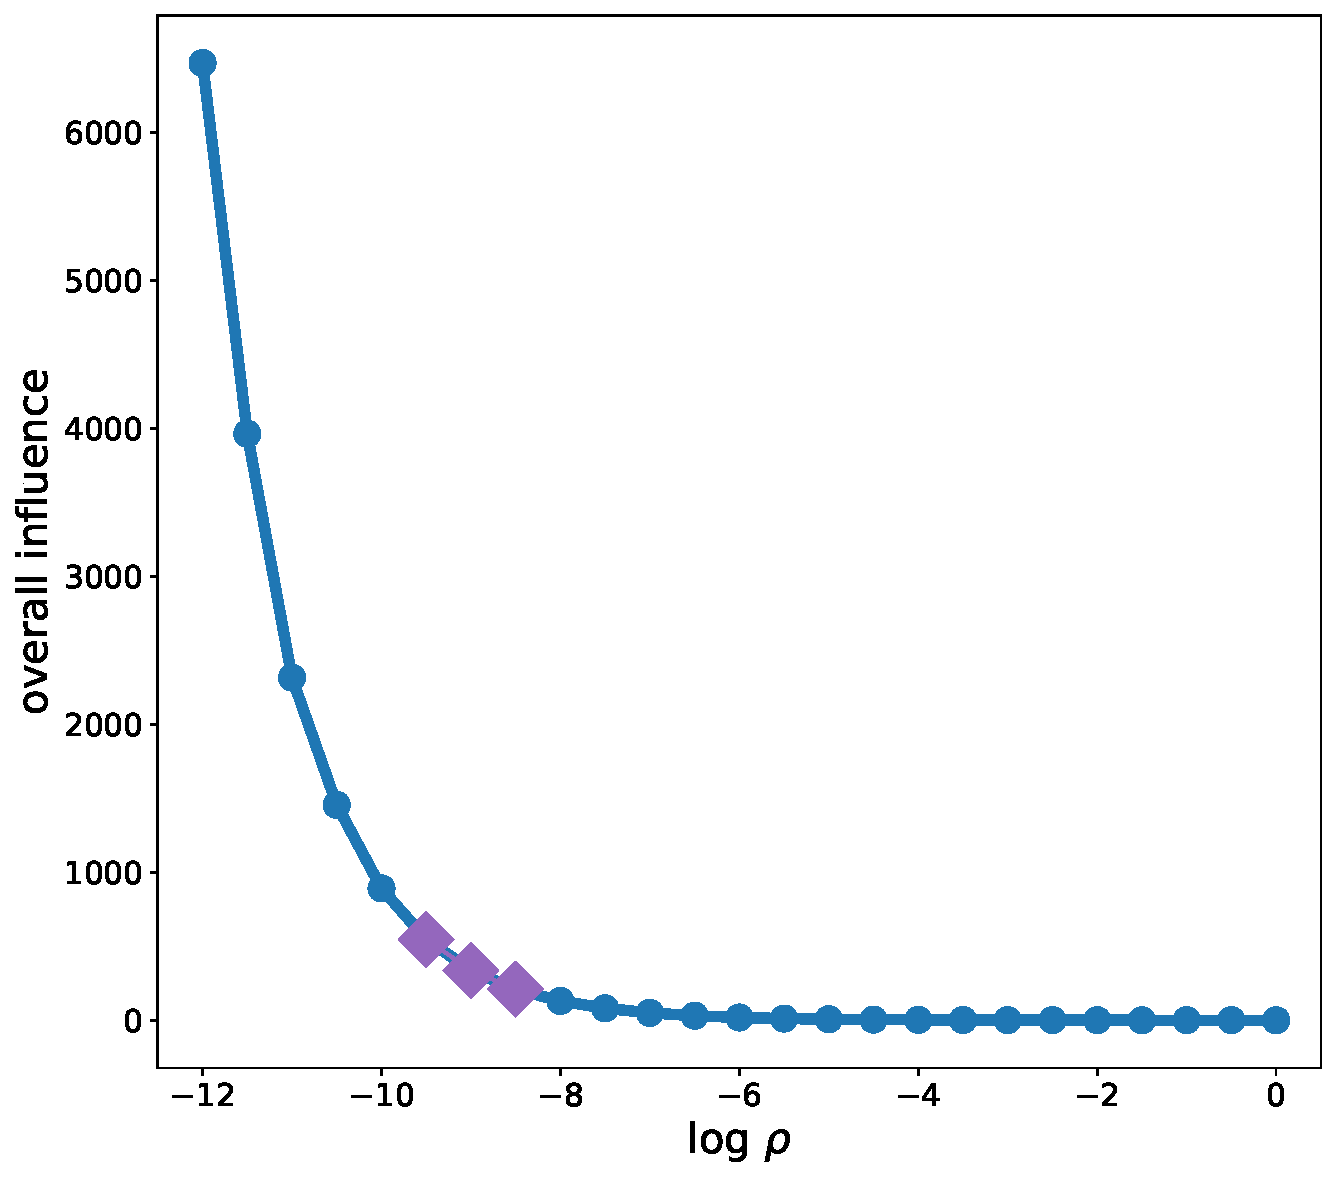
\includegraphics[width=0.7\textwidth]{../plots/waiting-SM-overall-empirical-influence-log-penalty-params-choose-best-baseden=Gamma-36-2-gridpoints=1-202-1.pdf}
%	\caption{XXXXX}
%	\label{fig-choose-appro-log-pen-param}
%\end{figure}
%
%In this plot, the points on the right end of the curve correspond to under-penalized SM density estimates that are very sensitive to the presence of $y$; and the the points on the left end of the curve correspond to over-penalized SM density estimates that are very insensitive to the presence of $y$. The points at the elbow corresponds to SM density estimates that are appropriately penalized. In this example, the points at the elbow (marked by purple diamonds) corresponds to $\rho = e^{-9.5}, e^{-9}$ and $e^{-8.5}$, and the corresponding penalized SM density estimates are shown in \textbf{\color{red}Figure \ref{XXXXXXX}}, which are all reasonable. 


\section{Which One to Use: Regularized Maximum Likelihood or Score Matching Density Estimators?}\label{section-which-one-to-use}

Now, we can compute penalized ML and regularized SM density estimators within $\calQ_{\ker}$. A natural question arises: which density estimator should one use? Regularized SM density estimators are easy to compute, and can be obtained by solving a linear system or adding and multiplying certain matrices, but are sensitive to the presence of isolated observations, especially when the amount of regularization is small. Penalized ML density estimator, on the other hand, is hard to compute as one has to handle $A$ and its derivative, but is \textit{not} very sensitive to the presence of isolated observations. We recommend to use regularized SM density estimators, primarily due to their computational advantage. When using them, one needs to impose an appropriate amount of regularization to ensure the resulting density estimate is not just a spike at the isolated observation or very close to the base density function $\mu$; otherwise, such a density estimate can be of no use and be misleading. One can use the $K$-fold cross-validation to select the appropriate amount of regularization as we did in this chapter and the earlier ones. % In terms of choosing between penalized and early stopping SM density estimators, we recommend the latter, again due to its computational advantage. 
